        %%******************************************%%
        %%                                          %%
        %%        Modello di tesi di laurea         %%
        %%            di Andrea Giraldin            %%
        %%                                          %%
        %%             2 novembre 2012              %%
        %%                                          %%
        %%******************************************%%


% I seguenti commenti speciali impostano:
% 1. 
% 2. PDFLaTeX come motore di composizione;
% 3. tesi.tex come documento principale;
% 4. il controllo ortografico italiano per l'editor.

% !TEX encoding = UTF-8
% !TEX TS-program = pdflatex
% !TEX root = tesi.tex
% !TEX spellcheck = it-IT

\documentclass[10pt,                    % corpo del font principale
               a4paper,                 % carta A4
               twoside,                 % impagina per fronte-retro
               openright,               % inizio capitoli a destra
               english,                 
               italian,                 
               ]{book}    

\usepackage[utf8]{inputenc}             % codifica di input; anche [latin1] va bene
                                        % NOTA BENE! va accordata con le preferenze dell'editor

%**************************************************************
% Importazione package
%************************************************************** 

\usepackage{placeins}

%\usepackage{amsmath,amssymb,amsthm}    % matematica

\usepackage[english, italian]{babel}    % per scrivere in italiano e in inglese;
                                        % l'ultima lingua (l'italiano) risulta predefinita

\usepackage{bookmark}                   % segnalibri

\usepackage{caption}                    % didascalie

\usepackage{chngpage,calc}              % centra il frontespizio

\usepackage{csquotes}                   % gestisce automaticamente i caratteri (")

\usepackage{emptypage}                  % pagine vuote senza testatina e piede di pagina

\usepackage{epigraph}					% per epigrafi

\usepackage{eurosym}                    % simbolo dell'euro

\usepackage[T1]{fontenc}                % codifica dei font:
                                        % NOTA BENE! richiede una distribuzione *completa* di LaTeX

%\usepackage{indentfirst}               % rientra il primo paragrafo di ogni sezione

\usepackage{graphicx}                   % immagini

\usepackage{hyperref}                   % collegamenti ipertestuali



\usepackage[binding=5mm]{layaureo}      % margini ottimizzati per l'A4; rilegatura di 5 mm

\usepackage{listings}                   % codici

\usepackage{microtype}                  % microtipografia

\usepackage{mparhack,fixltx2e,relsize}  % finezze tipografiche

\usepackage{nameref}                    % visualizza nome dei riferimenti                                      

\usepackage[font=small]{quoting}        % citazioni

\usepackage{subfig}                     % sottofigure, sottotabelle

\usepackage[italian]{varioref}          % riferimenti completi della pagina

\usepackage[dvipsnames]{xcolor}         % colori

\usepackage{booktabs}                   % tabelle                                       
\usepackage{tabularx}                   % tabelle di larghezza prefissata                                    
\usepackage{longtable}                  % tabelle su più pagine                                        
\usepackage{ltxtable}                   % tabelle su più pagine e adattabili in larghezza

\usepackage[toc, acronym]{glossaries}   % glossario
                                        % per includerlo nel documento bisogna:
                                        % 1. compilare una prima volta tesi.tex;
                                        % 2. eseguire: makeindex -s tesi.ist -t tesi.glg -o tesi.gls tesi.glo
                                        % 3. eseguire: makeindex -s tesi.ist -t tesi.alg -o tesi.acr tesi.acn
                                        % 4. compilare due volte tesi.tex.

\usepackage[backend=biber,style=verbose-ibid,hyperref,backref]{biblatex}
                                        % eccellente pacchetto per la bibliografia; 
                                        % produce uno stile di citazione autore-anno; 
                                        % lo stile "numeric-comp" produce riferimenti numerici
                                        % per includerlo nel documento bisogna:
                                        % 1. compilare una prima volta tesi.tex;
                                        % 2. eseguire: biber tesi
                                        % 3. compilare ancora tesi.tex.

\usepackage{listings}
\lstdefinestyle{sharpc}{language=[Sharp]C}

%**************************************************************
% file contenente le impostazioni della tesi
%**************************************************************

%**************************************************************
% Frontespizio
%**************************************************************
\newcommand{\myName}{Marco Prelaz}                              % autore
\newcommand{\myTitle}{Supporto e consulenza tecnica dell'applicativo NPS}                    
\newcommand{\myDegree}{Tesi di laurea triennale}                % tipo di tesi
\newcommand{\myUni}{Università degli Studi di Padova}           % università
\newcommand{\myFaculty}{Corso di Laurea in Informatica}         % facoltà
\newcommand{\myDepartment}{Dipartimento di Matematica}          % dipartimento
\newcommand{\myProf}{Mauro Conti}                               % relatore
\newcommand{\myLocation}{Padova}                                % dove
\newcommand{\myAA}{2015-2016}                                   % anno accademico
\newcommand{\myTime}{Dicembre 2016}                             % quando


%**************************************************************
% Impostazioni di impaginazione
% see: http://wwwcdf.pd.infn.it/AppuntiLinux/a2547.htm
%**************************************************************

\setlength{\parindent}{0pt}   % larghezza rientro della prima riga (era 14pt)
\setlength{\parskip}{0pt}   % distanza tra i paragrafi


%**************************************************************
% Impostazioni di biblatex
%**************************************************************
\bibliography{bibliografia} % database di biblatex 

\defbibheading{bibliography}
{
    \cleardoublepage
    \phantomsection 
    \addcontentsline{toc}{chapter}{\bibname}
    \chapter*{\bibname\markboth{\bibname}{\bibname}}
}

\setlength\bibitemsep{1.5\itemsep} % spazio tra entry

%\DeclareBibliographyCategory{opere}
\DeclareBibliographyCategory{web}

%\addtocategory{opere}{womak:lean-thinking}
\addtocategory{web}{site:wikipedia}
\addtocategory{web}{site:mediana}
\addtocategory{web}{site:msdn}
\addtocategory{web}{site:closedxml}
\addtocategory{web}{site:nps}

%\defbibheading{opere}{\section*{Riferimenti bibliografici}}
\defbibheading{web}{\section*{Siti Web consultati}}


%**************************************************************
% Impostazioni di caption
%**************************************************************
\captionsetup{
    tableposition=top,
    figureposition=bottom,
    font=small,
    format=hang,
    labelfont=bf
}

%**************************************************************
% Impostazioni di glossaries
%**************************************************************

%**************************************************************
% Acronimi
%**************************************************************
\renewcommand{\acronymname}{Acronimi}

%\newacronym[description={\glslink{apig}{Application Program Interface}}]
%    {api}{API}{Application Program Interface}

%\newacronym[description={\glslink{umlg}{Unified Modeling Language}}]
%    {uml}{UML}{Unified Modeling Language}
    
\newacronym[description={\glslink{itg}{Information Technology}}]
    {it}{IT}{Information Technology}
    
\newacronym[description={\glslink{sfag}{Sales Force Automation}}]
    {sfa}{SFA}{Sales Force Automation}
    
\newacronym[description={\glslink{crg}{Change Request}}]
    {cr}{CR}{Change Request}
    
\newacronym[description={\glslink{ideg}{Integrated Development Environment}}]
    {ide}{IDE}{Integrated Development Environment}   
   
\newacronym[description={\glslink{aspg}{Active Server Pages}}]
    {asp}{ASP}{Active Server Pages} 
    
\newacronym[description={\glslink{clrg}{Common Language Runtime}}]
    {clr}{CLR}{Common Language Runtime}      
    
\newacronym[description={\glslink{domg}{Common Language Runtime}}]
    {dom}{DOM}{Document Object Model}         
    
\newacronym[description={\glslink{sdkg}{Software Development Kit}}]
    {sdk}{SDK}{Software Development Kit}        

%**************************************************************
% Glossario
%**************************************************************
\renewcommand{\glossaryname}{Glossario}

%\newglossaryentry{apig}
%{
%    name=\glslink{api}{API},
%    sort=api,
%    description={in informatica con il termine \emph{Application Programming Interface API} (ing. interfaccia di programmazione di un'applicazione) si indica ogni insieme di procedure disponibili al programmatore, di solito raggruppate a formare un set di strumenti specifici per l'espletamento di un determinato compito all'interno di un certo programma. La finalità è ottenere un'astrazione, di solito tra l'hardware e il programmatore o tra software a basso e quello ad alto livello semplificando così il lavoro di programmazione}
%}

%\newglossaryentry{umlg}
%{
%    name=\glslink{uml}{UML},
%    sort=uml,
%    description={in ingegneria del software \emph{UML, Unified Modeling Language} (ing. linguaggio di modellazione unificato) è un linguaggio di modellazione e specifica basato sul paradigma object-oriented. L'\emph{UML} svolge un'importantissima funzione di ``lingua franca'' nella comunità della progettazione e programmazione a oggetti. Gran parte della letteratura di settore usa tale linguaggio per descrivere soluzioni analitiche e progettuali in modo sintetico e comprensibile a un vasto pubblico}
%}

\newglossaryentry{sfag}
{
    name=\glslink{sfa}{Sales Force Automation},
    sort=Sales Force Automation,
    description={In italiano corrisponde all'Automazione della Forza di Vendita, ovvero tutti gli applicativi aziendali di supporto alle vendite. Questi programmano e controllano l'azione dei venditori, li assistono nella messa a punto di un piano di vendita o di promozione di un determinato prodotto e sussidiano la raccolta degli ordini dei clienti}
}

\newglossaryentry{itg}
{
    name=\glslink{it}{Information Technology},
    sort=Information Technology,
    description={In italiano Tecnologia dell'Informazione, indica l'utilizzo di elaboratori e attrezzature di telecomunicazione per memorizzare, recuperare, trasmettere
e manipolare dati, spesso nel contesto di un'attività commerciale o di un'altra
impresa}
}

\newglossaryentry{system integrator}
{
    name=\glslink{system integrator}{System Integrator},
    text=system integrator,
    sort=system integrator,
    description={In italiano Integratore di Sistemi, è una tipologia di carriera nell'ambito dell'\gls{it}. In particolare gli integratori di sistemi devono essere molto capaci di conformare i prodotti esistenti ai bisogni del cliente}
}

\newglossaryentry{customer experience}
{
    name=\glslink{customer experience}{Customer Experience},
    text=customer experience,
    sort=customer experience,
    description={Soddisfazione del cliente in base alla sua esperienza di fronte a qualsiasi contatto diretto o indiretto con un'azienda}
}

\newglossaryentry{crg}
{
    name=\glslink{cr}{Change Request},
    sort=change request,
    description={Modifica da apportare ad un applicativo rispetto ai requisiti espressi dal cliente in fase di analisi},
    plural=Change Requests
}

\newglossaryentry{wireframe}
{
    name=\glslink{wireframe}{Wireframe},
    sort=wireframe,
    description={Bozza strutturale di un sito, applicativo web o \textit{software} che permette di individuare subito le dinamiche del progetto in termini di usabilità e utilizzo pratico, i punti critici e quelli che richiedono uno sviluppo più accurato o solamente alcuni miglioramenti},
    plural=wireframes
}

\newglossaryentry{mockup}
{
    name=\glslink{mockup}{Mockup},
    text=mockup,
    sort=mockup,
    description={Modello statico di una pagina web o \textit{mobile} molto dettagliato che viene costruito mediante \textit{software} grafico e che dovrà quindi essere implementato in quello che sarà l'applicativo finale},
    plural=mockups
}

\newglossaryentry{deliverable}
{
    name=\glslink{deliverable}{Deliverable},
    text=deliverable,
    sort=deliverable,
    description={Indica un risultato verificabile, di significativa rilevanza, che deve essere conseguito durante un progetto e fornito al committente},
    plural=deliverables
}

\newglossaryentry{ios}
{
    name=\glslink{ios}{iOS},
    sort=ios,
    description={Sistema operativo sviluppato da \textit{Apple} per \textit{iPhone}, \textit{iPod touch} e \textit{iPad}}
}

\newglossaryentry{android}
{
    name=\glslink{android}{Android},
    sort=android,
    description={Sistema operativo per dispositivi \textit{mobili} sviluppato da \textit{Google Inc.} e basato sul \textit{kernel} \textit{Linux}}
}

\newglossaryentry{ideg}
{
    name=\glslink{ide}{Integrated Development Environment},
    sort=Integrated Development Environment,
    description={In italiano Ambiente di Sviluppo Integrato, è un \textit{software} che aiuta i programmatori nello sviluppo del codice sorgente di un applicativo, tramite una serie di strumenti e funzionalità dedicate}
}

\newglossaryentry{aspg}
{
    name=\glslink{asp}{Active Server Pages},
    sort=Active Server Pages,
    description={Pagine web contenenti, oltre al puro codice HTML, degli \textit{script} che verranno elaborati lato server per generare il codice HTML \textit{runtime} da inviare al \textit{browser} dell'utente. In questo modo è possibile mostrare contenuti dinamici (ad esempio estratti da \textit{database} che risiedono sul server web) e modificarne l'aspetto secondo le regole programmate negli \textit{script}, il tutto senza dover inviare il codice del programma all'utente finale (al quale va inviato solo il risultato), con notevole risparmio di tempi e banda}
}

\newglossaryentry{clrg}
{
    name=\glslink{clr}{Common Language Runtime},
    sort=Common Language Runtime,
    description={Ambiente di \textit{runtime} fornito dal \textit{framework} .NET, in cui viene eseguito il codice  e nel quale sono offerti servizi (come la gestione della memoria, dei \textit{thread} e dei servizi remoti) che facilitano il processo di sviluppo. La base è costituita da un compilatore JIT (Just In Time). Ciò significa che il codice intermedio prodotto, identico per tutti i linguaggi di alto livello impiegati (supportati dal \textit{framework} .NET), viene compilato in linguaggio macchina al momento della prima esecuzione}
}

\newglossaryentry{domg}
{
    name=\glslink{dom}{Document Object Model},
    sort=Document Object Model,
    description={In italiano Modello a Oggetti del Documento, è una forma di rappresentazione dei documenti strutturati come modello orientato agli oggetti}
}

\newglossaryentry{intranet}
{
    name=\glslink{intranet}{Intranet},
    text=intranet,
    sort=intranet,
    description={Rete aziendale privata accessibile solamente al personale di quell'organizzazione}
}

\newglossaryentry{data model}
{
    name=\glslink{data model}{Data Model},
    text=data model,
    sort=data model,
    description={Modello astratto che indica come si relazionano fra loro i dati all'interno di un sistema, per questo a volte viene anche definito come struttura dati}
}

\newglossaryentry{sistema di ticketing}
{
    name=\glslink{sistema di ticketing}{Sistema di ticketing},
    text=sistema di ticketing,
    sort=sistema di ticketing,
    description={Sistema informatico che gestisce e registra delle liste di richieste di assistenza o di problemi, organizzato secondo le necessità di chi offre il servizio}
}

\newglossaryentry{screenshot}
{
    name=\glslink{screenshot}{Screenshot},
    text=screenshot,
    sort=screenshot,
    description={Un'immagine che rappresenta lo stato dello schermo del computer in un determinato istante}
}

\newglossaryentry{sdkg}
{
    name=\glslink{sdk}{Software Development Kit},
    sort=software development kit,
    description={In italiano Pacchetto di Sviluppo per Applicazioni, indica genericamente un insieme di strumenti per lo sviluppo e la documentazione di \textit{software}}
}

\newglossaryentry{stored procedure}
{
    name=\glslink{stored procedure}{Stored procedure},
    text=stored procedure,
    sort=stored procedure,
    description={Gruppi di istruzioni SQL compattati in un modulo e memorizzati nel \textit{database} stesso per un successivo utilizzo}
}

\newglossaryentry{diagramma di Gantt}
{
    name=\glslink{diagramma di Gantt}{Diagramma di Gantt},
    text=diagramma di Gantt,
    sort=diagramma di Gantt,
    description={Strumento di supporto alla gestione dei progetti, che rappresenta graficamente un calendario delle attività dando una chiara illustrazione dello stato d'avanzamento del progetto raffigurato}
}

\newglossaryentry{deployment}
{
    name=\glslink{deployment}{Deployment},
    text=deployment,
    sort=deployment,
    description={Consegna o rilascio al cliente, con relativa installazione e messa
in funzione di una applicazione o di un sistema software tipicamente all'interno di un sistema informatico aziendale}
}
 % database di termini
\makeglossaries


%**************************************************************
% Impostazioni di graphicx
%**************************************************************
\graphicspath{{immagini/}} % cartella dove sono riposte le immagini


%**************************************************************
% Impostazioni di hyperref
%**************************************************************
\hypersetup{
    %hyperfootnotes=false,
    %pdfpagelabels,
    %draft, % = elimina tutti i link (utile per stampe in bianco e nero)
    colorlinks=true,
    linktocpage=true,
    pdfstartpage=1,
    pdfstartview=FitV,
    % decommenta la riga seguente per avere link in nero (per esempio per la stampa in bianco e nero)
    %colorlinks=false, linktocpage=false, pdfborder={0 0 0}, pdfstartpage=1, pdfstartview=FitV,
    breaklinks=true,
    pdfpagemode=UseNone,
    pageanchor=true,
    pdfpagemode=UseOutlines,
    plainpages=false,
    bookmarksnumbered,
    bookmarksopen=true,
    bookmarksopenlevel=1,
    hypertexnames=true,
    pdfhighlight=/O,
    %nesting=true,
    %frenchlinks,
    urlcolor=webbrown,
    linkcolor=RoyalBlue,
    citecolor=webgreen,
    %pagecolor=RoyalBlue,
    %urlcolor=Black, linkcolor=Black, citecolor=Black, %pagecolor=Black,
    pdftitle={\myTitle},
    pdfauthor={\textcopyright\ \myName, \myUni, \myFaculty},
    pdfsubject={},
    pdfkeywords={},
    pdfcreator={pdfLaTeX},
    pdfproducer={LaTeX}
}

%**************************************************************
% Impostazioni di itemize
%**************************************************************
%\renewcommand{\labelitemi}{$\ast$}

\renewcommand{\labelitemi}{$\bullet$}
%\renewcommand{\labelitemii}{$\cdot$}
%\renewcommand{\labelitemiii}{$\diamond$}
%\renewcommand{\labelitemiv}{$\ast$}


%**************************************************************
% Impostazioni di listings
%**************************************************************
\lstset{
    language=[LaTeX]Tex,%C++,
    keywordstyle=\color{RoyalBlue}, %\bfseries,
    basicstyle=\small\ttfamily,
    %identifierstyle=\color{NavyBlue},
    commentstyle=\color{Green}\ttfamily,
    stringstyle=\rmfamily,
    numbers=none, %left,%
    numberstyle=\scriptsize, %\tiny
    stepnumber=5,
    numbersep=8pt,
    showstringspaces=false,
    breaklines=true,
    frameround=ftff,
    frame=single
} 


%**************************************************************
% Impostazioni di xcolor
%**************************************************************
\definecolor{webgreen}{rgb}{0,.5,0}
\definecolor{webbrown}{rgb}{.6,0,0}


%**************************************************************
% Altro
%**************************************************************

\newcommand{\omissis}{[\dots\negthinspace]} % produce [...]

% eccezioni all'algoritmo di sillabazione
\hyphenation
{
    ma-cro-istru-zio-ne
    gi-ral-din
}

\newcommand{\sectionname}{sezione}
\addto\captionsitalian{\renewcommand{\figurename}{figura}
                       \renewcommand{\tablename}{tabella}}

\newcommand{\glsfirstoccur}{\ap{{[g]}}}

\newcommand{\intro}[1]{\emph{\textsf{#1}}}

%**************************************************************
% Environment per ``rischi''
%**************************************************************
\newcounter{riskcounter}                % define a counter
\setcounter{riskcounter}{0}             % set the counter to some initial value

%%%% Parameters
% #1: Title
\newenvironment{risk}[1]{
    \refstepcounter{riskcounter}        % increment counter
    \par \noindent                      % start new paragraph
    \textbf{\arabic{riskcounter}. #1}   % display the title before the 
                                        % content of the environment is displayed 
}{
    \par\medskip
}

\newcommand{\riskname}{Rischio}

\newcommand{\riskdescription}[1]{\textbf{\\Descrizione:} #1.}

\newcommand{\risksolution}[1]{\textbf{\\Soluzione:} #1.}

%**************************************************************
% Environment per ``use case''
%**************************************************************
\newcounter{usecasecounter}             % define a counter
\setcounter{usecasecounter}{0}          % set the counter to some initial value

%%%% Parameters
% #1: ID
% #2: Nome
\newenvironment{usecase}[2]{
    \renewcommand{\theusecasecounter}{\usecasename #1}  % this is where the display of 
                                                        % the counter is overwritten/modified
    \refstepcounter{usecasecounter}             % increment counter
    \vspace{10pt}
    \par \noindent                              % start new paragraph
    {\large \textbf{\usecasename #1: #2}}       % display the title before the 
                                                % content of the environment is displayed 
    \medskip
}{
    \medskip
}

\newcommand{\usecasename}{UC}

\newcommand{\usecaseactors}[1]{\textbf{\\Attori Principali:} #1. \vspace{4pt}}
\newcommand{\usecasepre}[1]{\textbf{\\Precondizioni:} #1. \vspace{4pt}}
\newcommand{\usecasedesc}[1]{\textbf{\\Descrizione:} #1. \vspace{4pt}}
\newcommand{\usecasepost}[1]{\textbf{\\Postcondizioni:} #1. \vspace{4pt}}
\newcommand{\usecasealt}[1]{\textbf{\\Scenario Alternativo:} #1. \vspace{4pt}}

%**************************************************************
% Environment per ``namespace description''
%**************************************************************

\newenvironment{namespacedesc}{
    \vspace{10pt}
    \par \noindent                              % start new paragraph
    \begin{description} 
}{
    \end{description}
    \medskip
}

\newcommand{\classdesc}[2]{\item[\textbf{#1:}] #2}                     % file con le impostazioni personali

\begin{document}
%**************************************************************
% Materiale iniziale
%**************************************************************
\frontmatter
% !TEX encoding = UTF-8
% !TEX TS-program = pdflatex
% !TEX root = ../tesi.tex
% !TEX spellcheck = it-IT

%**************************************************************
% Frontespizio 
%**************************************************************
\begin{titlepage}

\begin{center}

\begin{LARGE}
\textbf{\myUni}\\
\end{LARGE}

\vspace{10pt}

\begin{figure}[htbp]
\begin{center}

\includegraphics[height=30pt]{logoDM}
\end{center}
\end{figure}

\begin{large}
\textsc{\myFaculty}\\
\end{large}

\vspace{25pt}
\begin{figure}[htbp]
\begin{center}

\includegraphics[height=6cm]{logo-unipd}
\end{center}
\end{figure}
\vspace{5pt} 

\begin{LARGE}
\begin{center}
\textbf{\myTitle}\\
\end{center}
\end{LARGE}

\vspace{10pt} 

\begin{large}
\textsl{\myDegree}\\
\end{large}

\vspace{70pt} 

\begin{large}
\textit{Relatore}
\hfill
\textit{Laureando}\\
\vspace{5pt} 
Prof. \myProf
\hfill
\myName
\end{large}

\vspace{40pt}

\line(1, 0){338} \\
\begin{normalsize}
\textsc{Anno Accademico \myAA}
\end{normalsize}

\end{center}
\end{titlepage} 
% !TEX encoding = UTF-8
% !TEX TS-program = pdflatex
% !TEX root = ../tesi.tex
% !TEX spellcheck = it-IT

%**************************************************************
% Colophon
%**************************************************************
\clearpage
\phantomsection
\thispagestyle{empty}

\hfill

\vfill

\noindent\myName: \textit{\myTitle,}
\myDegree,
\textcopyright\ \myTime.
% !TEX encoding = UTF-8
% !TEX TS-program = pdflatex
% !TEX root = ../tesi.tex
% !TEX spellcheck = it-IT

%**************************************************************
% Dedica
%**************************************************************
\cleardoublepage
\phantomsection
\thispagestyle{empty}
\pdfbookmark{Dedica}{Dedica}

\vspace*{3cm}

\medskip

\begin{center}
Dedicato alla mia famiglia.
\end{center}

% !TEX encoding = UTF-8
% !TEX TS-program = pdflatex
% !TEX root = ../tesi.tex
% !TEX spellcheck = it-IT

%**************************************************************
% Sommario
%**************************************************************
\cleardoublepage
\phantomsection
\pdfbookmark{Sommario}{Sommario}
\begingroup
\let\clearpage\relax
\let\cleardoublepage\relax
\let\cleardoublepage\relax

\chapter*{Sommario}
Il presente documento descrive il lavoro svolto durante il periodo di stage, della durata complessiva di 303 ore, dal laureando Marco Prelaz presso l'azienda Mediana S.r.l.u.   

Nel primo capitolo darò una breve panoramica sull'azienda che mi ha ospitato, specificando inoltre quali sono i prodotti e i servizi che offre alla sua clientela.
%concentrandomi maggiormente sugli aspetti che ho potuto vedere di persona (o con i quali ho avuto a che fare). 

L'oggetto del secondo capitolo sarà invece il progetto nel quale sono stato inserito durante questo tirocinio. Fornirò quindi una visione dettagliata dell'applicativo, capendo da che tipo di esigenze nasce e quali sono le funzionalità principali che vengono proposte.
 
Nel terzo capitolo invece racconterò lo stage stesso partendo dal calendario delle attività svolte, per passare poi alla descrizione delle diverse fasi che hanno caratterizzato questo tirocinio e che hanno permesso di soddisfare gli obiettivi inizialmente proposti.

L'ultima parte di questa relazione conterrà un consuntivo sul mio lavoro e un confronto con la panificazione iniziale. Inoltre esporrò le conclusioni personali sull'esperienza vissuta, un resoconto delle conoscenze acquisite e la mia visione del corso di laurea in funzione delle impressioni avute dal mondo del lavoro.

%\vfill
%
%\selectlanguage{english}
%\pdfbookmark{Abstract}{Abstract}
%\chapter*{Abstract}
%
%\selectlanguage{italian}

\endgroup			

\vfill


% !TEX encoding = UTF-8
% !TEX TS-program = pdflatex
% !TEX root = ../tesi.tex
% !TEX spellcheck = it-IT

%**************************************************************
% Ringraziamenti
%**************************************************************
\cleardoublepage
\phantomsection
\pdfbookmark{Ringraziamenti}{ringraziamenti}

%\begin{flushright}{
%	\slshape    
%	``Life is really simple, but we insist on making it complicated''} \\ 
%	\medskip
%    --- Confucius
%\end{flushright}


\bigskip

\begingroup
\let\clearpage\relax
\let\cleardoublepage\relax
\let\cleardoublepage\relax

\chapter*{Ringraziamenti}

\textit{Innanzitutto, vorrei esprimere la mia gratitudine al Professore Mauro Conti, relatore della mia tesi, per l'aiuto e il sostegno fornitomi durante la stesura di questa relazione finale.}\\

\textit{Desidero ringraziare con affetto i miei genitori per aver sempre creduto in me, per aver supportato ogni mia decisione e per essermi stati vicini anche nei momenti più difficili.}\\

\textit{Ringrazio poi il mio tutor aziendale Davide Bacelle per avermi condotto durante questa esperienza lavorativa e per essere stato sempre disponibile a rispondere ad ogni mio dubbio. Insieme a lui ringrazio anche tutti gli altri colleghi di Mediana S.r.l.u., che mi hanno accolto fin da subito nel migliore dei modi.}\\

\textit{Voglio infine ringraziare tutti i miei amici, a partire dal mio amico d'infanzia Massimo che mi sopporta ancora, i compagni del liceo Giacomo e Andrea con i quali sono rimasto particolarmente legato, la squadra di calcetto con la quale sfogarsi giocando a pallone e i miei colleghi universitari e in particolar modo il mio team di Ingegneria del Software con il quale ho passato momenti indimenticabili.}\\
\bigskip

\textit{\myLocation, \myTime}
\hfill \myName

\endgroup


% !TEX encoding = UTF-8
% !TEX TS-program = pdflatex
% !TEX root = ../tesi.tex
% !TEX spellcheck = it-IT

%**************************************************************
% Indici
%**************************************************************
\cleardoublepage
\pdfbookmark{\contentsname}{tableofcontents}
\setcounter{tocdepth}{2}
\tableofcontents
%\markboth{\contentsname}{\contentsname} 
\clearpage

\begingroup 
    \let\clearpage\relax
    \let\cleardoublepage\relax
    \let\cleardoublepage\relax
    %*******************************************************
    % Elenco delle figure
    %*******************************************************    
    \phantomsection
    \pdfbookmark{\listfigurename}{lof}
    \listoffigures

    \vspace*{8ex}

    %*******************************************************
    % Elenco delle tabelle
    %*******************************************************
    \phantomsection
    \pdfbookmark{\listtablename}{lot}
    \listoftables
        
    \vspace*{8ex}
\endgroup

\cleardoublepage

\cleardoublepage

%**************************************************************
% Materiale principale
%**************************************************************
\mainmatter
% !TEX encoding = UTF-8
% !TEX TS-program = pdflatex
% !TEX root = ../tesi.tex
% !TEX spellcheck = it-IT

%**************************************************************
\chapter{Il contesto aziendale}
\label{cap:contesto-aziendale}
%**************************************************************

%\noindent Esempio di citazione in linea \\
%\cite{site:mediana}. \\

%\noindent Esempio di citazione nel pie' di pagina \\
%citazione\footcite{site:mediana} \\


%\begin{description}
%    \item[{\hyperref[cap:processi-metodologie]{Il secondo capitolo}}] descrive ...
    
%    \item[{\hyperref[cap:descrizione-stage]{Il terzo capitolo}}] approfondisce ...
    
%    \item[{\hyperref[cap:analisi-requisiti]{Il quarto capitolo}}] approfondisce ...
    
%    \item[{\hyperref[cap:progettazione-codifica]{Il quinto capitolo}}] approfondisce ..
    
%    \item[{\hyperref[cap:verifica-validazione]{Il sesto capitolo}}] approfondisce ...
    
%    \item[{\hyperref[cap:conclusioni]{Nel settimo capitolo}}] descrive ...
%\end{description}

%**************************************************************
\section{L'azienda}
\label{azienda}

Mediana S.r.l.u.(logo nella \hyperref[logoMediana]{Figura 1.1}) è una realtà aziendale nata nel 1994 con sede a Padova. Fondata nel pieno del boom dell'\acrshort{it} e all'inizio della diffusione su larga scala della connessione Internet, Mediana S.r.l.u. vuole imporsi sin da subito nel nuovo mercato dello sviluppo software. Inizialmente legata prettamente alla \acrshort{sfa}, con la liberalizzazione del mercato dell'energia l'azienda ha saputo rinnovarsi specializzandosi in modo deciso in un settore che presenta peculiarità tecniche, legislative e burocratiche, sviluppando prodotti specifici legati alla fatturazione dell'energia elettrica e del gas. Sebbene questo settore costituisca ancora il \textit{business core} dell'azienda, con il passare del tempo Mediana S.r.l.u. sta ampliando i propri orizzonti. Da un lato infatti i prodotti tradizionali legati al mondo dell'energia si stanno arricchendo di valore grazie all'apporto di nuove conoscenze ed esperienza. Dall'altro la nuova frontiera è rappresentata dalle soluzioni destinate all'utente finale, ovvero sia lo sviluppo di applicativi di gestione del \textit{business}, sia la realizzazione di strumenti di analisi per creare valore nella \gls{customer experience}. Forte di un'esperienza ventennale su campo nazionale e internazionale, Mediana S.r.l.u. ha sviluppato competenze specifiche ed evolvendosi dalla semplice vendita del prodotto \textit{software} al ruolo di \gls{system integrator} ha potuto garantire continuità nel rapporto con i propri clienti focalizzando il lavoro del proprio \textit{team} su un servizio di consulenza personalizzato.

\begin{figure}[ht]
\begin{center}

\includegraphics[height=50pt]{mediana_logo}
\caption{Logo Mediana S.r.l.u.}
\label{logoMediana}
\end{center}
\end{figure}

%**************************************************************
\clearpage
\section{Organizzazione aziendale}
\label{organizzazione}

L'azienda si compone di figure con competenze di tipo tecniche e amministrative diverse che possono assumere i seguenti ruoli:
\begin{itemize}
	\item\textbf{Project Manager}: gestisce le risorse e gli eventi del progetto. Essendo il punto di riferimento per l'intero progetto, è responsabile di tempi, costi e qualità del risultato finale. Si occupa infine di gestire eventuali \acrshort{cr} e fraintendimenti sulle specifiche di progetto;
	\item\textbf{Consulente business}: individua ambito ed obiettivi di progetto, verifica la sua fattibilità e tramite incontri di \textit{business} analisi con il cliente formalizza i requisiti. Deve essere poi in grado di far emergere le esigenze del cliente nell'ambito del progetto, al di là di quelle meramente espresse, in modo che la definizione del progetto che andrà a descrivere sia la più completa possibile;
	\item\textbf{Consulente tecnico}: crea il modello informatico della realtà di \textit{business}, verificando innanzitutto la fattibilità tecnica del progetto e facendo in seguito una stima dei tempi e delle risorse necessarie. Deve inoltre essere in grado di creare nuove configurazioni e inserire/modificare i dati degli utenti attraverso strumenti di manipolazione diretta dei dati come SQL. È necessario quindi che conosca le logiche di funzionamento delle applicazioni per le quali svolge questo ruolo;
	\item\textbf{Sviluppatore}: scrive \textit{software} nell'ambiente di sviluppo e nel \textit{database} scelto per l'applicazione seguendo le linee guida e gli standard definiti in azienda. Esegue inoltre i test di unità delle funzionalità che ha sviluppato;
	\item\textbf{Web designer}: realizza elaborati grafici di interfacce web, tablet, mobile che dovranno essere compatibili con la successiva implementazione da parte del \textit{team} di sviluppo. In continuo confronto sia con quest'ultimo che con il committente produce quindi dei \glspl{wireframe} per definire la struttura, gli elementi e il comportamento delle interfacce. Realizza infine dei \glspl{mockup} dettagliati che devono essere valutati e approvati dal committente e successivamente implementati dal \textit{team} di sviluppo. Offre inoltre supporto nella realizzazione di presentazioni volte alla promozione dei prodotti e servizi offerti dall'azienda.
\end{itemize}

Nella \hyperref[organigramma]{Figura 1.2} è possibile vedere una panoramica su come sono legati fra loro i ruoli appena descritti. Questi, a seconda delle esigenze, è probabile che vengano associati alla stessa persona, che quindi risulta avere diversi incarichi anche durante l'arco di vita dello stesso progetto.

\begin{figure}[ht]
\begin{center}
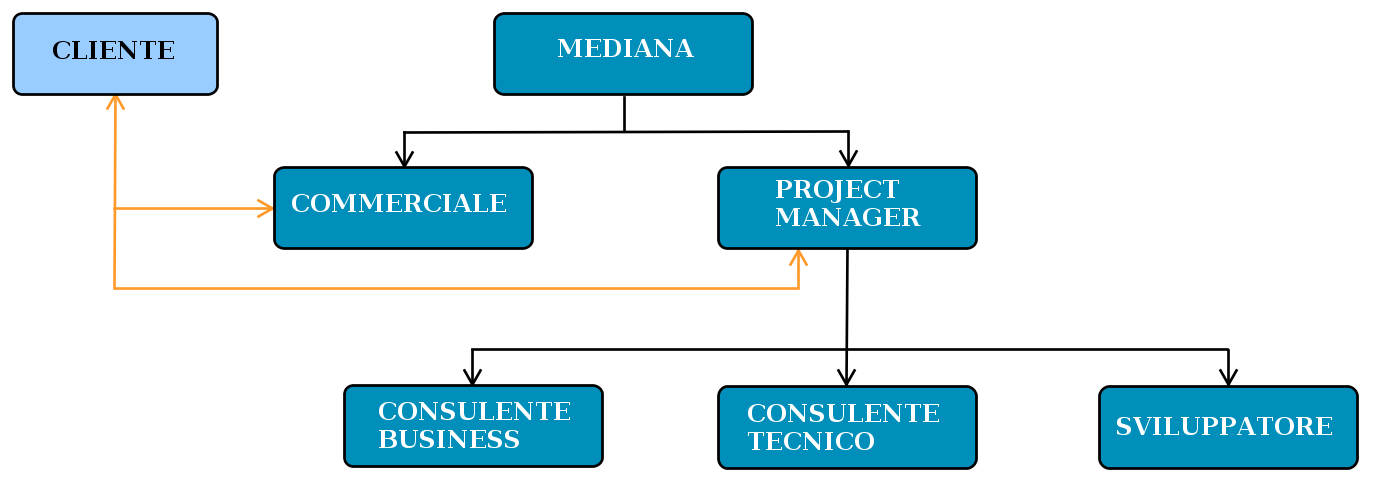
\includegraphics[scale=0.35]{OrganigrammaMediana}
\caption{Organizzazione per progetto in Mediana S.r.l.u.}
\label{organigramma}
\end{center}
\end{figure}
\FloatBarrier

%**************************************************************
\section{Prodotti aziendali}
\label{prodotti}

I prodotti di punta che l'azienda Mediana S.r.l.u. offre alla sua clientela sono:

\begin{itemize}
\item \textbf{XEnergy}: \textit{software} dedicato alle aziende che operano nel mondo dell'energia elettrica e gas, permette la gestione della fatturazione, dei preventivi, delle anagrafiche dei clienti e delle offerte, oltre che il controllo prezzo nella vendita sempre al passo con le novità di mercato e normative;
\item \textbf{XContract}: \textit{software} dedicato alla \acrshort{sfa}, permette l'inserimento e la gestione dei contratti per la vendita di energia elettrica e gas. Consente la corretta gestione del punto di fornitura, dall'inserimento a sistema all'attivazione del contratto, garantendo le tempistiche e il rispetto delle normative dell'Autorità garante per l'energia elettrica e gas;
\item \textbf{Web Portal}: \textit{software} che fornisce agli utenti delle aziende legate al mondo dell'energia elettrica e gas strumenti per monitorare lo stato delle loro fatture, consumi e contratti, sia tramite web che \textit{apps} \gls{ios} e \gls{android};
\item \textbf{CSIndex}: \textit{software} che consente di raccogliere il voto ed il feedback sia dei clienti di un'azienda che vende prodotti/servizi sia dei propri dipendenti (come descritto più approfonditamente nel \hyperref[cap:progetto-stage]{secondo capitolo}); permette poi di gestire le informazioni, visualizzare grafici ed estrazioni in base ai dati raccolti.
\end{itemize}

%**************************************************************
\section{Processi interni}
\label{processi}

In questa sezione descrivo il modello di ciclo di vita del \textit{software} utilizzato dall'azienda, le fasi che contraddistinguono un progetto dall'idea del cliente fino alla consegna del risultato finale. 

\subsection{Modello di ciclo di vita del software}
\label{ciclo di vita}
Nel fornire i progetti ex novo o effettuando cambiamenti evolutivi, Mediana S.r.l.u. segue un approccio incrementale che vede l'esecuzione delle fasi standard per macro \glspl{deliverable}. Viene quindi adottato un modello a spirale (rappresentato nella \hyperref[spirale]{Figura 1.3}) che abbraccia prototipazione, sviluppo iterativo del \textit{software}, e la valutazione del rischio. In questo modo lo sviluppo può essere arrestato alla fine di ogni ciclo a seconda della valutazione del ciclo precedente.

\begin{figure}[ht]
\begin{center}
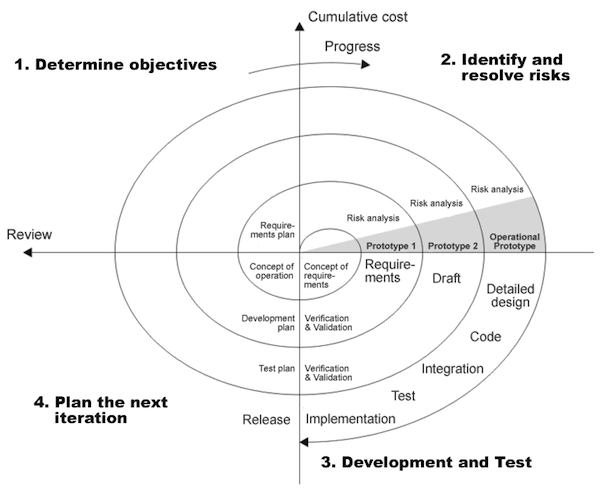
\includegraphics[scale=0.4]{ModelloSpirale}
\caption{Rappresentazione del modello di sviluppo a spirale}
\label{spirale}
\end{center}
\end{figure}
\FloatBarrier

\subsection{Le fasi di un progetto}
\label{fasi progetto}
Adesso vado ad analizzare le fasi che accompagnano la realizzazione di un progetto in Mediana S.r.l.u., specificando per ognuna di esse quali sono i documenti che le caratterizzano:

\begin{enumerate}
\item Una prima idea viene proposta al dipartimento \acrshort{it} dell'azienda cliente che redige un primo documento chiamato \textbf{Bill of Requirements} (\textbf{B.O.R.}) nel quale vengono riassunti i requisiti in modo molto generico;
\item Nella \textbf{Functional Analysis} (in caso di un nuovo prodotto) o \textbf{Gap Analysis} (nel caso di un'espansione di un prodotto già esistente) si analizza il \textbf{B.O.R.} per capire cosa si è in grado di realizzare e si fa quindi una prima stima di tempi e costi presentando una bozza delle possibili funzionalità che in futuro verranno sviluppate;
\item Si provvede poi a presentare un \textbf{documento di offerta} al cliente, contenente i costi e i tempi definitivi;
\item Approvata l'offerta viene creato un \textbf{diagramma di Gantt} al fine di pianificare, coordinare e tracciare le varie attività del progetto, che quindi viene ufficialmente lanciato (\textbf{Kick-off});
\item Mediana S.r.l.u. provvede quindi a redigere un documento, che dovrà essere confermato dal cliente, intitolato \textbf{Business Blue Print} (\textbf{B.B.P.}), nel quale vengono presentati i \glspl{mockup} e tutti i dettagli delle varie funzionalità che verranno poi implementate;
\item In seguito, con il cliente, si effettueranno regolarmente dei controlli per verificare che vengano rispettati i tempi come da pianificazione, riportando i dettagli nello \textbf{Stato di avanzamento dei lavori} (\textbf{S.A.L.});
\item Nella fase conclusiva del progetto vengono redatti gli \textbf{User Acceptance Test} (\textbf{U.A.T.}), con i quali Mediana S.r.l.u. conduce il cliente nell'effettuare, passo per passo, i test alle diverse funzionalità del \textit{software} in questione. In questo modo il cliente può verificare che l'applicativo funzioni correttamente;
\item In seguito, nel \textbf{Sir recap}, verranno segnalati tutti gli eventuali \textit{bug} da correggere o le \acrshort{cr} che sono sorte durante la fase di \textit{testing}. In base all'entità delle modifiche effettuate, o se ritenuto necessario, verranno ripetuti gli \textbf{U.A.T.};
\item Infine vengono redatti tutti i \textbf{manuali} necessari all'utente finale per comprendere al meglio il \textit{software} che dovrà utilizzare. Questi vengono consegnati al cliente durante la fase di prova del \textit{software} che da lì a breve verrà rilasciato in produzione.
\end{enumerate}

La \hyperref[fasiProgetto]{Figura 1.4} riassume tutte le fasi appena descritte, identificandole in base alla documentazione che le contraddistingue.

\begin{figure}[ht]
\begin{center}
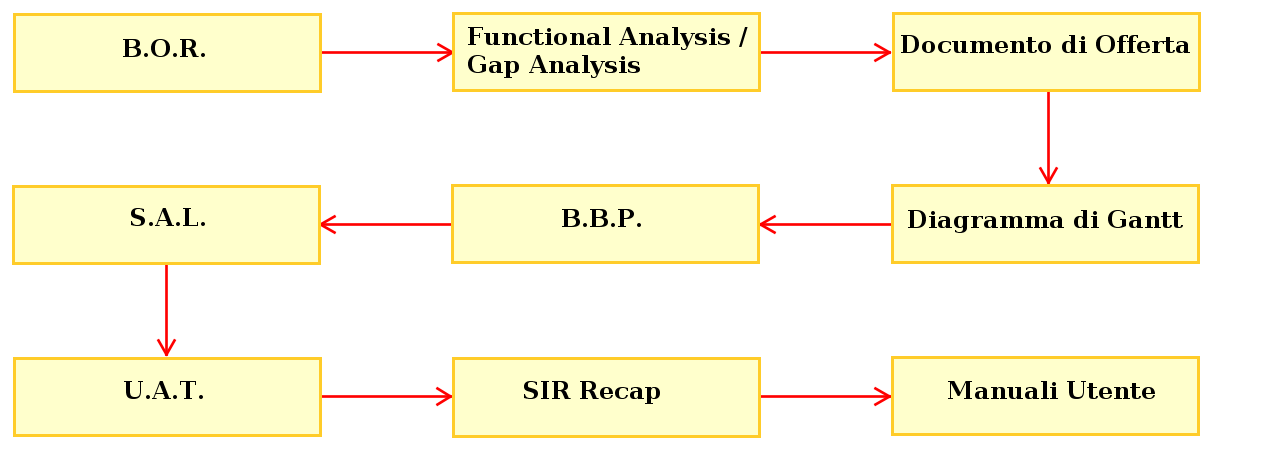
\includegraphics[scale=0.40]{FasiProgettoMediana}
\caption{Fasi di un progetto in Mediana S.r.l.u.}
\label{fasiProgetto}
\end{center}
\end{figure}
\FloatBarrier

\subsection{Ambienti di un programma}
\label{ambienti programma}
In base alla fase del progetto che si è raggiunta, il \textit{team} di Mediana S.r.l.u. rilascia i suoi \textit{software} nei seguenti ambienti così definiti:
\begin{itemize}
\item \textbf{Develoment environment (DEV)}: ambiente dove i programmatori creano le nuove applicazioni o aggiungono le nuove funzionalità richieste, tramite \acrshort{cr}, dal committente;
\item \textbf{Quality Assurance environment (QA)}: ambiente di test dove anche il committente può provare le funzionalità dell'applicativo concluso o aggiornato;
\item \textbf{Production environment (PROD)}: ambiente dove l'applicazione, che è stata approvata definitivamente dal committente, diventa fruibile all'utente finale.
\end{itemize}

\section{Strumenti e tecnologie a supporto dello sviluppo}
\label{strumenti e tecnologie}
Mediana S.r.l.u., nel sviluppare i propri \textit{software}, utilizza diversi strumenti e tecnologie.

\subsection{Sistemi operativi}
\label{sistemi operativi}
Il personale di Mediana S.r.l.u. utilizza per la maggior parte sistemi operativi \textbf{Windows}, salvo rari casi nei quali vengono utilizzati sistemi operativi \textbf{Mac OS} installati su macchine \textit{iMac} o \textit{MacBook Pro}.

\subsection{Tecnologie utilizzate}
\label{tecnologie}
Nella maggior parte dei progetti, Mediana S.r.l.u. utilizza le seguenti tecnologie:
\begin{itemize}
\item \textbf{ASP.NET}: insieme di tecnologie di sviluppo di \textit{software} per il web, commercializzate da \textit{Microsoft}. Sebbene il nome ASP.NET derivi da \acrshort{asp} (la vecchia tecnologia per lo sviluppo web di \textit{Microsoft}), esistono sostanziali differenze fra le due. Infatti ASP.NET si basa, come tutte le applicazioni della famiglia \textit{Microsoft} .NET, sul \acrshort{clr}. Le applicazioni ASP.NET sono significativamente più veloci e performanti rispetto a quelle realizzate utilizzando altre tecnologie di \textit{scripting}, in quanto l'intero codice del sito web è pre-compilato in pochi file \textit{dll} gestiti da un \textit{web server}. ASP.NET è progettato in modo da incoraggiare lo sviluppatore ad usare in modo sistematico il paradigma dell'interfaccia grafica abbinato alla cosiddetta programmazione ad eventi, cioè allo stile di programmazione in cui i vari blocchi di codice vengono eseguiti in risposta a determinati eventi su controlli dotati di rappresentazione grafica;
\item \textbf{HTML}: linguaggio di programmazione, e più nello specifico linguaggio di \textit{mark-up}, utilizzato per descrive il contenuto di una pagina web;
\item \textbf{CSS}: linguaggio usato per definire la formattazione delle pagine che costituisco un sito web, andando nello specifico a modificare il \textit{layout} di queste;
\item \textbf{Javascript}: linguaggio di \textit{scripting} orientato agli oggetti e agli eventi, comunemente utilizzato nella programmazione web lato \textit{client} per la creazione, in siti web e applicazioni web, di effetti dinamici interattivi. La caratteristica principale di JavaScript è quella di non essere un linguaggio compilato bensì interpretato. Viene utilizzato principalmente per scrivere piccole funzioni che vengono integrate nelle pagine HTML e che interagiscono con il \acrshort{dom} del browser per compiere determinate azioni non possibili con il solo HTML statico, come controllare i valori nei campi di ingresso, ecc.;
\item \textbf{C\#}: linguaggio di programmazione orientato agli oggetti sviluppato da \textit{Microsoft} all'interno dell'iniziativa .NET. La sintassi del C\# prende spunto da quella del Delphi (hanno il medesimo autore), del C++, di Java e anche in parte di Visual Basic per gli strumenti di programmazione visuale e per la sua semplicità;
\item \textbf{Transact-SQL}: versione proprietaria del linguaggio SQL sviluppata da \textit{Microsoft}, che ne estende le prestazioni aumentando:
\begin{itemize}
\item Funzioni per controllo di flusso;
\item Possibilità di definire variabili locali;
\item Varie funzioni per la manipolazione di stringhe ed altre tipologie di dati;
\item Possibilità di aggiungere, all'opzione \textit{FROM}, una \textit{JOIN} che permetta il collegamento tra più tabelle anche nelle operazioni di \textit{DELETE} e \textit{UPDATE}.
\end{itemize}
\end{itemize}

\subsection{Ambienti di sviluppo}
\label{ambienti sviluppo}
Gli \acrshort{ide} che vengono utilizzati per produrre il codice sono:
\begin{itemize}
\item \textbf{Microsoft Visual Studio}: ambiente sviluppato da \textit{Microsoft}, che supporta tutti i linguaggi legati al \textit{framework} .NET (compresi C\#, HTML e Javascript) e che permette la realizzazione di applicazioni, siti web, applicazioni web e servizi web.  Permette inoltre di correggere eventuali errori sintattici (ed alcuni logici) senza compilare l'applicativo, possiede poi un debugger interno per il rilevamento e la correzione degli errori logici nel codice in \textit{runtime} e fornisce diversi strumenti per l'analisi prestazionale;
\item \textbf{Microsoft SQL Server Management Studio}: ambiente pensato per l'accesso, la configurazione, la gestione, l'amministrazione e lo sviluppo di tutti i componenti di \textit{Microsoft SQL Server}. SQL Server Management Studio integra un'ampia gamma di strumenti grafici e editor di script avanzati per eseguire operazioni all'interno di \textit{database}. Tramite il cosiddetto \textit{Object Explorer} è poi possibile navigare, selezionare, e modificare tutti gli oggetti presenti all'interno dell'istanza di \textit{Microsoft SQL Server} (come per esempio \textit{database}, tabelle, ecc.).
\end{itemize}

\subsection{Software di versionamento}
\label{sw verionamento}
Vista la sua facile integrazione con il \textit{tool} di sviluppo \textit{Visual Studio}, Mediana S.r.l.u. ha deciso di adottare come \textit{software} per la gestione delle versioni dei suoi programmi \textbf{Microsoft Visual Sourcesafe}. Questo prodotto viene utilizzato per il controllo delle versioni a livello di \textit{file}, ciò consente al \textit{team} di utilizzare più versioni di un progetto contemporaneamente in modo da gestire versioni di codice parallele. Le funzionalità principali che Visual SourceSafe offre sono:
\begin{itemize}
\item Protezione del \textit{team} dalle perdite accidentali di \textit{file};
\item Controllo delle versioni precedenti di un \textit{file};
\item Supporto della diramazione, della condivisione, dell'unione e della gestione di versioni di \textit{file};
\item Controllo delle versioni di interi progetti;
\item Controllo di codice modulare (un \textit{file} riutilizzato, o condiviso, in più progetti).
\end{itemize}

\subsection{Software per la documentazione}
\label{sw documentazione}
Per la stesura di tutta le documentazione interna, ma anche per quella condivisa con i clienti e per quella destinata all'utente finale (come possono essere per esempio i manuali utente), Mediana S.r.l.u. utilizza \textbf{Microsoft Word}; uno dei programmi del suo genere più diffusi al mondo.

\subsection{Applicativi di supporto alla comunicazione e aggiornamento del lavoro}
\label{sw comunicazione}
Per tutte le comunicazioni interne si utilizzano le \textbf{e-mail} aziendali che vengono fornite al momento dell'assunzione; mentre per avere un continuo aggiornamento sullo stato dei lavori vengono condivisi dei documenti o fogli di calcolo online tramite \textbf{Google Drive}, un potente servizio di condivisione dati che consente il lavoro concorrente su di uno stesso \textit{file}.             % Introduzione
% !TEX encoding = UTF-8
% !TEX TS-program = pdflatex
% !TEX root = ../tesi.tex
% !TEX spellcheck = it-IT

%**************************************************************
\chapter{Il progetto di stage}
\label{cap:progetto-stage}
%**************************************************************

% \intro{Brevissima introduzione al capitolo}\\

%**************************************************************
\section{Introduzione al progetto}
Il progetto sul quale è stato incentrato il mio stage presso Mediana S.r.l.u. è stato \textbf{NPS EBS}, ovvero una variante del già citato CSIndex per il cliente \textbf{E.ON Business Services} (EBS). Il nome NPS si rifà invece alla nota tipologia di indagine \textbf{Net Promoter Score} nella sua variante dedicata ai dipendenti (eNPS).

\section{Il concetto eNPS}
\label{concetto eNPS}
L'idea di base nasce da una semplice considerazione: ascoltare il giudizio del cliente non è sufficiente a migliorare nel lungo termine la \gls{customer experience}, ma è necessario considerare anche le opinioni ed il \textit{feedback} dei propri dipendenti. Quest'ultimi sono coloro che osservano giornalmente le reazioni dei clienti, ma anche coloro che gestiscono le interazioni e che comprendono e conoscono i processi operativi, avendo il potere di formare le esperienze dei clienti. Quindi se l'esperienza dei dipendenti è negativa, questi finiranno per mettere a serio rischio la relazione con i clienti. \\
Per questo motivo, per implementare un corretto programma che risponda a queste esigenze, è necessario definire innanzitutto una metrica chiara. Una delle più utilizzate è per l'appunto l'eNPS (Employee Net Promoter Score), apprezzabile sia per la sua semplicità che per la sua immediatezza. Infatti come per la metodologia NPS classica, ideata per ascoltare le opinioni del cliente, si basa sulle risposte date ad una semplice domanda:
\begin{center}
\emph{Su una scala da 0 a 10, con quale probabilità consiglieresti questa azienda come posto di lavoro?}
\end{center}
I dipendenti possono essere quindi suddivisi in tre categorie:
\begin{itemize}
\item \textbf{Promotori}: coloro che hanno dato un voto pari a 9 o 10;
\item \textbf{Passivi}: coloro che hanno dato un voto pari a 7 o 8;
\item \textbf{Detrattori}: coloro che hanno dato un voto che va da 0 a 6.
\end{itemize}
A questo punto il punteggio NPS viene calcolato, come rappresentato anche nella \hyperref[NPS]{Figura 2.1} secondo questa formula:
\begin{center}
$ NPS = \%Promotori - \%Detrattori $
\end{center}

\begin{figure}[ht]
\begin{center}
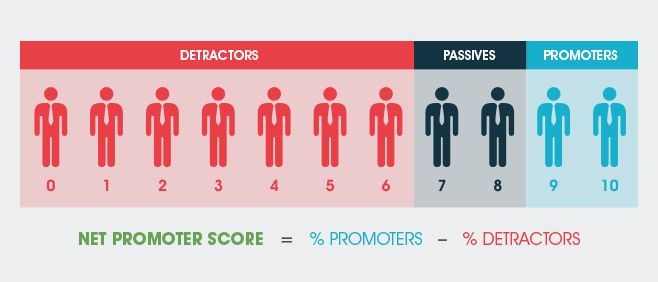
\includegraphics[scale=0.55]{NPS}
\caption{Net Promoter Score (NPS)}
\label{NPS}
\end{center}
\end{figure}
\FloatBarrier

In aggiunta a questo quesito non deve però mancare anche un'altra domanda a risposta aperta:
\begin{center}
\emph{Quali sono le ragioni del tuo voto?}
\end{center}
Solo in questo modo infatti è davvero possibile riuscire a cogliere le indicazioni e consigli che i dipendenti vorranno dare. 
%Infatti delle semplici domande a risposta chiusa costringono i rispondenti a schemi prefissati che rispecchiano sì il modo di vedere dell’organizzazione ma che non colgono di certo gli aspetti non ancora esplorati.

\section{Il progetto NPS EBS}
Sulla base di quanto espresso nella \hyperref[concetto eNPS]{Sezione 2.2}, l'E.ON Business Services (EBS) di Hannover (Germania) (logo nella \hyperref[EON]{Figura 2.2}) ha richiesto a Mediana S.r.l.u. un applicativo per gestire \textit{web survey} in moda da calcolare l'eNPS ed analizzare i dati in base ai \textit{feedback} raccolti.

\begin{figure}[ht]
\begin{center}

\includegraphics[height=45pt]{eon}
\caption{Logo del committente E.ON}
\label{EON}
\end{center}
\end{figure}

\subsection{Tipi di indagine}
Sono previsti tre differenti approcci nell'effettuare le indagini d'interesse:
\begin{itemize}
\item \textbf{Top-down}: permette ai dipendenti delle diverse sedi di EBS di dare un giudizio sui vari reparti che lo costituiscono (\textit{Human Resource}, \textit{Finance}, \acrshort{it}, ecc.) o sui servizi interni offerti;
\item \textbf{Bottom-up}: permette ai dipendenti di E.ON, che hanno avuto un interazione con EBS per risolvere alcuni problemi, di dare un giudizio sulla qualità del lavoro che in quel particolare caso è stato svolto;
\item \textbf{Passive}: permette a tutti i dipendenti di E.ON di dare un giudizio generico e anonimo su EBS.
\end{itemize}
Per quanto riguarda i primi due approcci la prima operazione da cui partire per poter effettuare le indagini d'interesse è il recupero delle informazioni sui potenziali intervistati. Per poter scegliere i contatti con i quali interagire è necessario prima caricare i dati anagrafici dei dipendenti.
% e gli eventuali \textit{touchpoint}.
Questa operazione, che viene effettuate dall'amministratore quando necessaria, fa si che il sistema NPS memorizzi o aggiorni, all'interno del proprio \textit{database}, i dati dei vari contatti che successivamente potranno essere selezionati nel caso l'esigenza dell'indagine lo richieda. \\
Terminata la fase di \textit{upload} dei contatti si passa appunto alla fase di selezione dove il responsabile dell'indagine può scegliere le persone, che verranno poi interpellate tramite una \textit{survey}, caricando nell'apposita sezione un \textit{file} CSV che rispetti la struttura concordata con il cliente oppure selezionandoli da una lista all'interno dell'applicativo. Queste prima di essere confermate dovranno superare i criteri dell'algoritmo, che permettono di evitare il verificarsi di situazioni che potrebbero infastidire gli intervistati. \\
Nello specifico i controlli fatti sono i seguenti:
\begin{itemize}
\item \textbf{Quality Control}: nel caso vengano selezionati dei contatti non presenti nel sistema o presenti più volte nello stesso \textit{file} CSV o quant'altro, questi vengono scartati;
\item \textbf{Blacklist}: nel caso vengano selezionati dei contatti che erano stati inseriti in precedenza nella \textit{blacklist} (per esempio quelli che hanno fatto richiesta di non voler più essere contattati per le indagini), questi vengono scartati;
\item \textbf{Obsolescenza}: nel caso vengano selezionati contatti che hanno ricevuto già una \textit{survey} nel breve periodo (predefinito) questi vengono scartati;
\item \textbf{Undercapacity}: nel caso venga selezionato un numero minore di contatti rispetto al numero minimo di \textit{survey} richieste per un così detto \textit{target group/touchpoint} (l'obbiettivo di studio di un indagine), tutti i contatti vengono scartati;
\item \textbf{Overcapacity}: nel caso venga selezionato un numero maggiore di contatti appartenenti ad una particolare sezione di EBS 
%(definiti nell'applicativo come \textit{Resolver Group Team}) 
rispetto al numero massimo di \textit{survey} gestibili da ogni responsabile di queste aree, vengono scartati i contatti che hanno una priorità minore rispetto a quella degli altri.
\end{itemize}
L'applicativo procede automaticamente con l'invio delle \textit{e-mail}, le cui parti sono personalizzabili dagli amministratori del sistema in un'apposita sezione del programma. In ogni \textit{e-mail} è presente un \textit{link} ad una \textit{web survey} che contiene, in base all'approccio, le rispettive domande NPS nelle quali gli intervistati possono sia dare un voto che giustificare, se essi lo vorranno, la risposta data in un apposito spazio. \'E infine presente un \textit{flag} che permette di dare il consenso di essere ricontattati per una così detta \textbf{second call}, che sarà utile per capire più approfonditamente le ragioni del giudizio che è stato dato.
In ogni momento, da quando un destinatario di queste \textit{e-mail} inizia a compilare una \textit{survey}, può decidere di interrompere momentaneamente la sua compilazione pur non avendola completata e ultimarla soltanto in un secondo momento. Se la \textit{survey} scade e non è stata ancora completata allora viene chiusa e tutti i dati parziali che erano stati immessi vengono cancellati; mentre se fin dall'inizio viene ignorata allora il sistema invia una nuova \textit{e-mail} di promemoria. Il periodo di attesa prima dell'invio della \textit{e-mail} di promemoria e la data di scadenza di una \textit{survey} possono essere configurate in una schermata apposita dell'applicativo NPS. I \textit{feedback} vengono dunque registrati nel sistema e viene tenuta traccia di tutti i dettagli dall'invio delle \textit{e-mail} fino alla conferma di compilazione completata, quindi non solo le risposte date ma anche lo stato delle \textit{survey} e le date di interesse come quelle di emissione e quelle nel quale vengono confermati i \textit{feedback} dai dipendenti.\\
L'approccio \textbf{Passive} permette invece a chiunque abbia accesso all'EBS \gls{intranet} di accedere tramite un apposito \textit{link} ad una \textit{web survey} che, a differenza degli altri due approcci appena visti, darà la possibilità di rispondere al quesito NPS in modo del tutto anonimo, presentandosi visivamente come nella \hyperref[Passive]{Figura 2.3}. Per questo motivo il sistema è in grado di riconoscere l'origine diversa del feedback registrandolo in modo che esso sia poi distinguibile dagli altri. Nel caso si volesse essere ricontattati per una \textbf{second call}, basterà comunque inserire in un' apposita sezione della \textit{survey} l'identificativo con il quale si è registrati all'interno dell'applicazione NPS, perdendo però in questo modo l'anonimato. 

\begin{figure}[ht]
\begin{center}
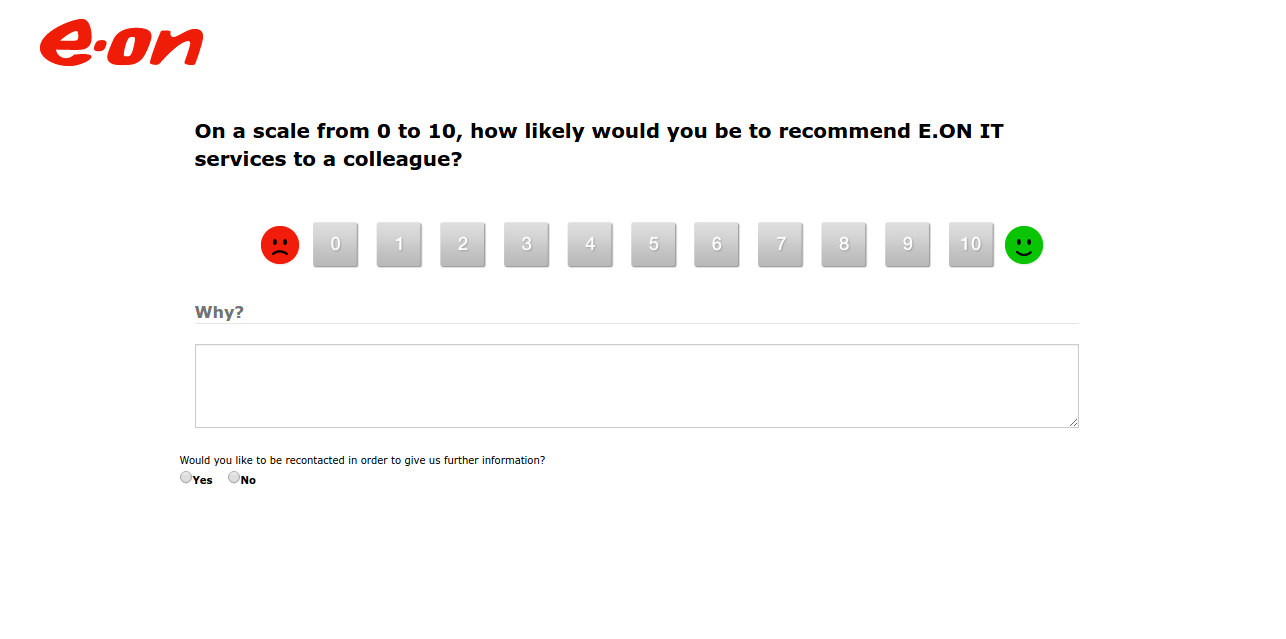
\includegraphics[scale=0.34]{PassiveSurvey}
\caption{Esempio di survey utilizzando un approccio Passive}
\label{Passive}
\end{center}
\end{figure}
\FloatBarrier

\subsection{Categorizzazione}

Per ogni \textit{feedback} raccolto dalle \textit{survey} viene data la possibilità di condurre una categorizzazione su quattro livelli (opzionali) in una maschera dedicata:\begin{enumerate}
\item \textbf{Type}: categoria che descrive il tipo di \textit{feedback}, ovvero in concreto se questo corrisponde a una segnalazione negativa, un complimento o un suggerimento;
\item \textbf{Class}: categoria che descrive in modo generico il contenuto del \textit{feedback} (per esempio "sostituzione hardware");
\item \textbf{Topic}: sotto-categoria legata strettamente a quella esposta nel punto precedente che la descrive più nel dettaglio (prendendo per buono l'esempio "sostituzione hardware" qui potrebbe essere "laptop","schermo PC","cellulare",ecc.);
\item \textbf{Reasons}: categoria che descrive le motivazioni che hanno spinto a rilasciare quel voto.
\end{enumerate}
Il responsabile di ogni sezione di EBS potrà visualizzare e quindi classificare, nel modo definito precedentemente, soltanto i \textit{feedback} della propria area di competenza. Nella stessa maschera, visibile nella \hyperref[Categorization]{Figura 2.4}, sarà inoltre possibile riportare per iscritto gli eventuali chiarimenti effettuati tramite le \textit{call}, che potranno a loro volta essere categorizzate.

\begin{figure}[h!]
\begin{center}
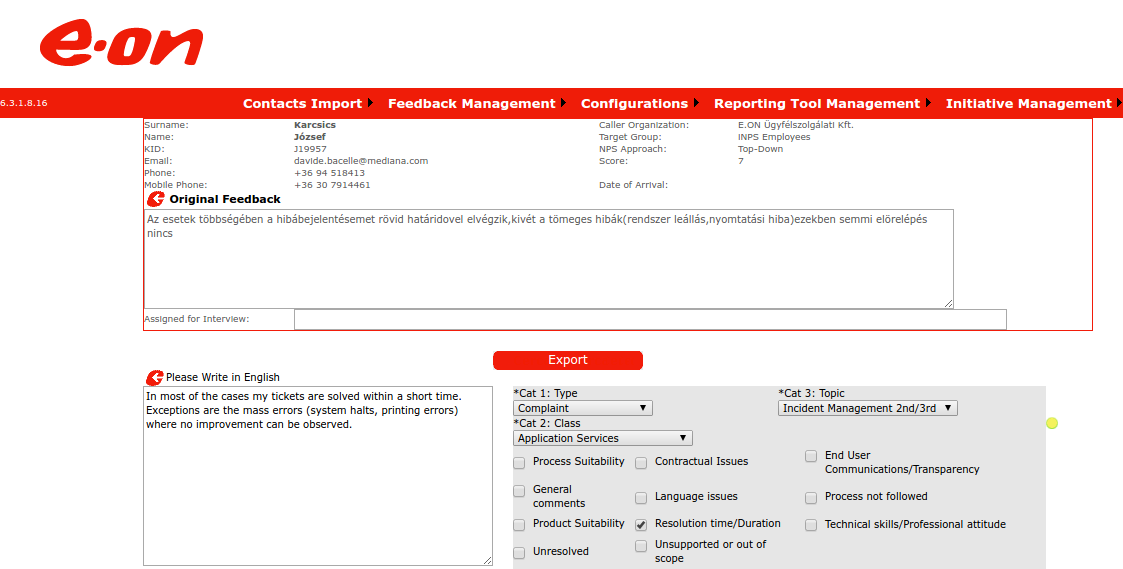
\includegraphics[scale=0.34]{FeedbackCategorized}
\caption{Esempio di feedback categorizzato}
\label{Categorization}
\end{center}
\end{figure}
\FloatBarrier

In questa sezione infine ogni \textit{feedback} può assumere tre stati differenti:
\begin{itemize}
\item \textbf{To Do}: \textit{feedback} rilasciati che non sono ancora stati categorizzati dalla persona addetta a tale operazione;
\item \textbf{Draft}: \textit{feedback} categorizzati solo in parte o comunque da rivedere prima di essere salvati definitivamente;
\item \textbf{Categorized}: \textit{feedback} categorizzati in modo definitivo e quindi non più modificabili.
\end{itemize}

\subsection{Reportistica}
\label{reporting tool}
I punteggi e i \textit{feedback} che sono stati memorizzati all'interno del \textit{database}, possono essere visualizzati tramite grafici che permetto all'utente di analizzare le varie statistiche nel modo più semplice possibile. \\
Esistono tre tipologie differenti di grafico:
\begin{itemize}
\item \textbf{Grafico a linee}: indicato per analizzare l'andamento temporale di una particolare statistica;
\item \textbf{Grafico a barre}: indicato per analizzare la distribuzione di una particolare statistica;
\item \textbf{Grafico a torta}: indicato per avere una visione d'insieme di una particolare statistica (esempio nella \hyperref[torta]{Figura 2.5}).
\end{itemize}

\begin{figure}[h!]
\begin{center}
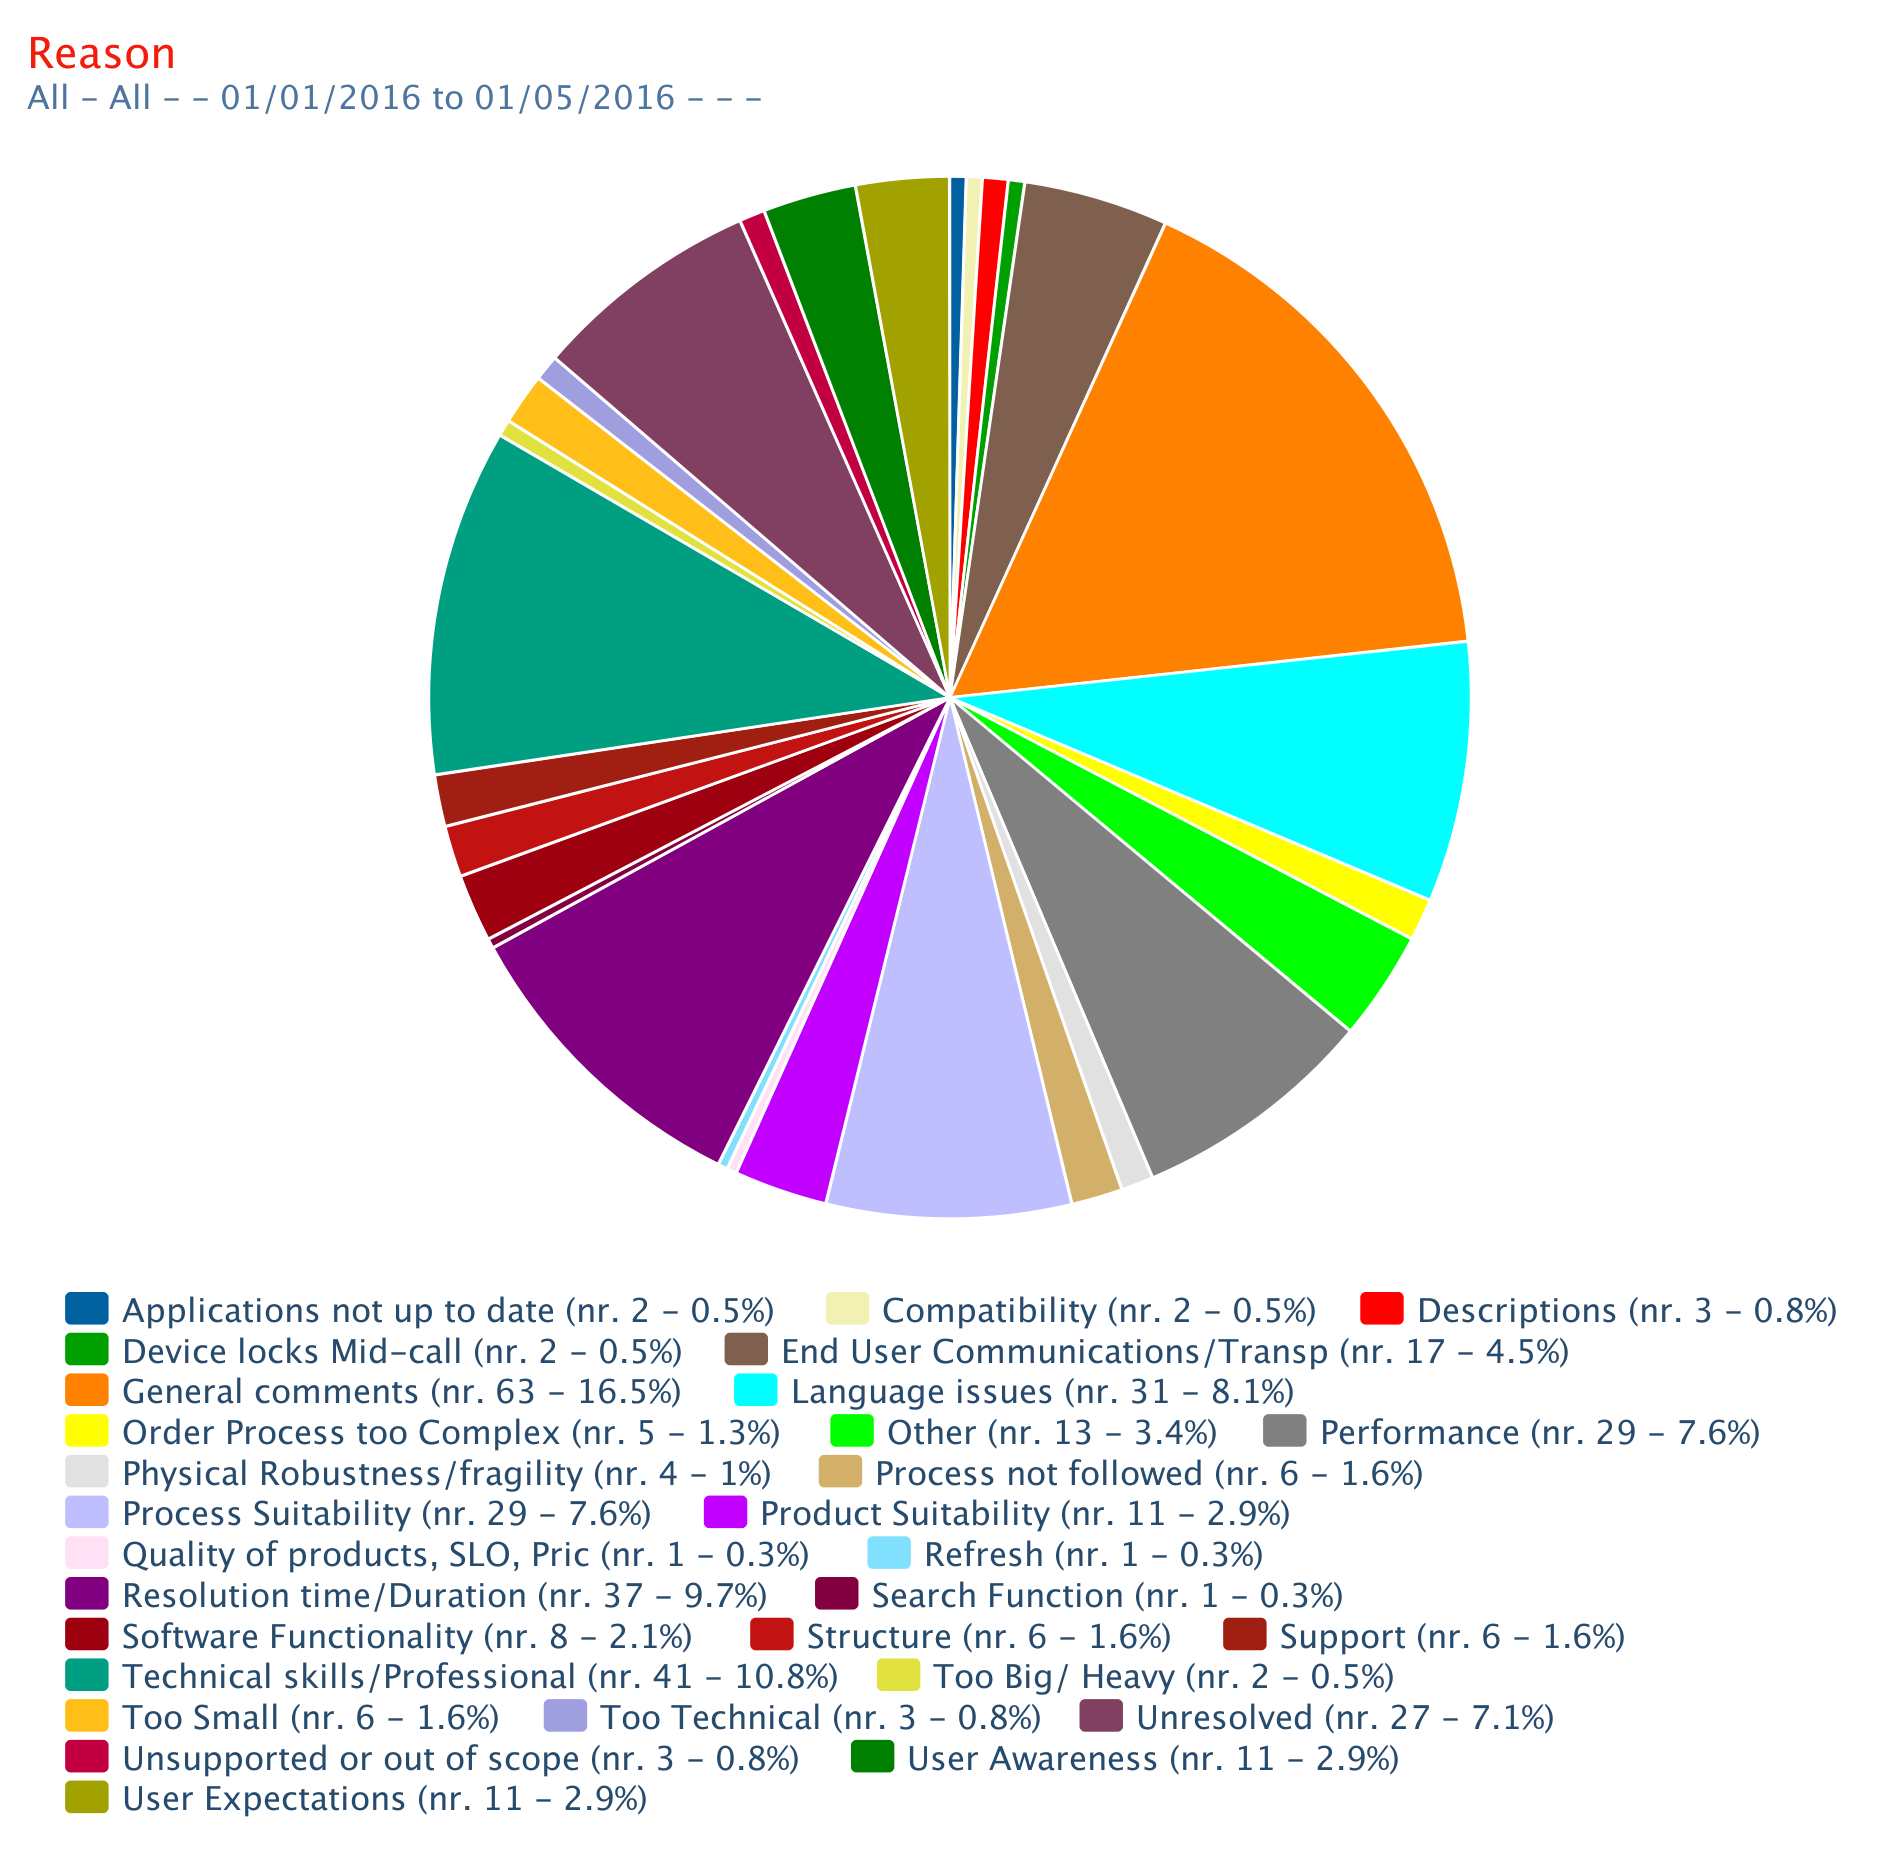
\includegraphics[scale=0.2]{GraficoTorta}
\caption{Esempio di grafico a torta}
\label{torta}
\end{center}
\end{figure}
\FloatBarrier

Questa pagina del programma NPS mette inoltre a disposizione le seguenti funzionalità e caratteristiche: 
\begin{itemize}
\item \textbf{Filtri}: utili per selezionare soltanto i dati di reale interesse, per esempio permettono di selezionare il periodo, la granularità, l'approccio delle \textit{survey} e le categorie dei \textit{feedback};
\item \textbf{Stampa e Download}: è possibile esportare il grafico in formato JPEG, PNG, SVG (formato vettoriale) e PDF oppure stamparlo direttamente dalla pagina web;
\item \textbf{Legenda dinamica}: cliccando le voci della legenda si possono togliere/aggiungere dal grafico i dati selezionati;
\item \textbf{Labels}: passando sopra con il mouse nelle diverse parti che compongono un grafico, è possibile ottenere informazioni dettagliate su queste;
\item \textbf{Zoom}: strumento che permette di visualizzare il grafico ingrandito in una finestra \textit{pop-up};
\item \textbf{Chiusura/Apertura Grafico}: strumento che permette di nascondere il grafico all'interno della pagina (tramite lo stesso bottone è poi possibile riaprirlo).
\end{itemize}

\subsection{Iniziative}
L'iniziativa è un'azione intrapresa da EBS con lo scopo di migliorare la soddisfazione del suo organico. Questa è verificabile attraverso l'invio di successive \textit{survey} sullo stesso argomento.\\
La necessità di programmare una nuova iniziativa parte dall'analisi fatta in seguito
alla raccolta dei dati con le \textit{survey}.\\
Individuata la categoria bisognosa di un intervento è necessario passare
all'approfondimento dei singoli \textit{feedback} per poter capire in che modo migliorare il servizio.\\
L'iniziativa può assumere tre differenti stati:
\begin{itemize}
\item \textbf{Draft}: l'iniziativa non è ancora ben definita ed è ancora modificabile;
\item \textbf{Open}: l'iniziativa è partita e non è più modificabile;
\item \textbf{Closed}: l'iniziativa è conclusa.
\end{itemize}

Terminata la creazione di una iniziativa è possibile collegarla ai \textit{feedback} di interesse e se desiderato inviare al contatto una \textit{e-mail} che lo informa sull'iniziativa intrapresa dall'azienda per migliorare la situazione.

\subsection{Impostazioni e personalizzazioni}
Senza entrare troppo nello specifico adesso elenco le molteplici sezioni che permettono una corretta configurazione della struttura e dei parametri del sistema NPS:
\begin{itemize}
\item È possibile abilitare nuovi utenti e assegnare loro uno dei ruoli previsti all'interno del sistema, a seconda delle funzioni alle quali essi possano accedere;
\item Tutte le domande, le \textit{label} e i messaggi delle \textit{survey}, oltre al corpo e l'oggetto delle \textit{e-mail}, possono essere personalizzate per definire il testo che leggeranno gli intervistati;
\item Per verificare di aver settato nel modo desiderato le impostazioni specificate nel punto precedente, l'applicativo NPS prevede una funzione dove è possibile inviare una \textit{e-mail} con una \textit{survey} di prova a un determinato indirizzo di posta elettronica;
\item Aggiungere, modificare o eliminare il possibile contenuto delle varie categorie che permettono di classificare i \textit{feedback};
\item Configurare nuovi \textit{target group/touchpoint}, che corrispondono allo scopo per le quali vengono fatte partire le indagini d'interesse, specificando parametri come per esempio il tipo di approccio da utilizzare, il periodo di validità della \textit{survey}, le opzioni di categorizzazione possibili, ecc.
\end{itemize} 
             % Processi
% !TEX encoding = UTF-8
% !TEX TS-program = pdflatex
% !TEX root = ../tesi.tex
% !TEX spellcheck = it-IT

%**************************************************************
\chapter{Descrizione dello stage}
\label{cap:descrizione-stage}
%**************************************************************

%\intro{Breve introduzione al capitolo}\\

%**************************************************************
%\section{Analisi preventiva dei rischi}

%Durante la fase di analisi iniziale sono stati individuati alcuni possibili rischi a cui si potrà andare incontro.
%Si è quindi proceduto a elaborare delle possibili soluzioni per far fronte a tali rischi.\\

%\begin{risk}{Performance del simulatore hardware}
%    \riskdescription{le performance del simulatore hardware e la comunicazione con questo potrebbero risultare lenti o non abbastanza buoni da causare il fallimento dei test}
%    \risksolution{coinvolgimento del responsabile a capo del progetto relativo il simulatore hardware}
%    \label{risk:hardware-simulator} 
%\end{risk}

%**************************************************************
\section{Obiettivi dello stage}
\label{obiettivi}
Sulla base della durata dello stage, l'azienda ha fissato degli obiettivi che si aspettava di veder raggiunti entro il termine del rapporto lavorativo. In particolare veniva richiesta:
\begin{itemize}
\item Conoscenza degli applicativi di Mediana S.r.l.u., in particolare di CSIndex nella sua ultima versione NPS EBS;
\item Conoscenza delle fasi consulenziali come:
	\begin{itemize}
	\item Redazione di \textit{test book} per U.A.T.\footnotemark[1];
	\item Test e verifiche dei programmi presi in esame;
	\item Redazione di manuali propedeutici al \textit{roll out} dell'applicativo.
	\end{itemize}
\item Apprendimento del \gls{data model} di NPS EBS;
\item Sviluppare una buona autonomia nella progettazione e sviluppo di \textit{statement} SQL.
\end{itemize}

\section{Calendario delle attività}
\label{calendario}
Nel dettaglio il lavoro è stato suddiviso nel seguente modo:
\begin{enumerate}
\item \textbf{Settimana 1}: introduzione ai prodotti aziendali e alla metodologie di lavoro in Mediana S.r.l.u.;
\item \textbf{Settimana 2}: focalizzazione sul prodotto NPS EBS e condivisione della documentazione inerente a questo progetto;
\item \textbf{Settimana 3}: esecuzione dei test funzionali descritti negli U.A.T in affiancamento al tutor;
\footnotetext[1]{Test visti in un punto della \hyperref[fasi progetto]{Sezione 1.4.2}}
\item \textbf{Settimana 4}: aggiornamento dei manuali per le diverse categorie di utente previste all'interno dell'applicativo;
\item \textbf{Settimana 5-6}: conoscenza del codice dell'applicativo e della struttura del \textit{database} in affiancamento agli sviluppatori;
\item \textbf{Settimana 7-8}: \textit{support} di NPS EBS fino al rilascio in PROD\footnotemark[2] 
\footnotetext[2]{Uno degli ambienti trattati nella \hyperref[ambienti programma]{Sezione 1.4.3}};
\end{enumerate}

Per una più chiara panoramica di questa suddivisione, nella \hyperref[gantt attivita]{Figura 3.1} riporto il \gls{diagramma di Gantt} con il calendario di tutte le attività svolte durante il periodo di stage.

\begin{figure}[h!]
\begin{center}
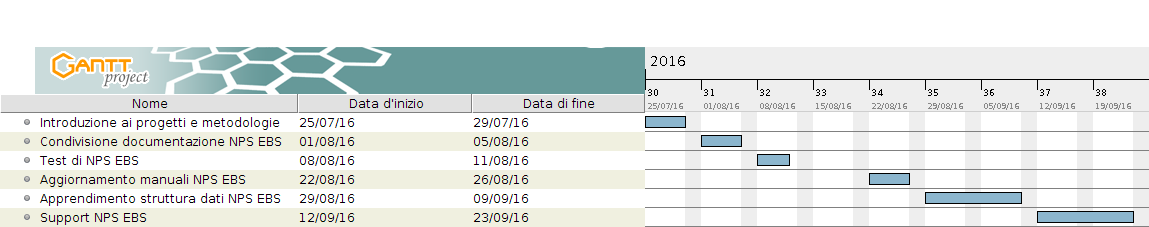
\includegraphics[scale=0.32]{Gantt} 
\caption{Diagramma di Gantt delle attività svolte}
\label{gantt attivita}
\end{center}
\end{figure}
\FloatBarrier

\section{Suddivisione dello stage e motivo della scelta}
Dal calendario si evince che lo stage è stato caratterizzato da due periodi distinti che sono identificabili nel modo seguente:
\begin{itemize}
\item Le prime quattro settimane sono servite inizialmente per apprendere il lavoro di consulente tecnico per poi metterlo in pratica con test e stesura dei manuali utente;
\item Le ultime quattro settimane invece sono state contraddistinte da un lavoro che si addice più che altro a uno sviluppatore, infatti tramite alcune operazioni di \textit{bug-fixing} ho potuto metter mano sia al codice, apprendendo così parte della logica che costituisce il programma NPS, sia al \textit{database}, capendo come vengono strutturati e suddivisi i dati che costituiscono il sistema.
\end{itemize}
Questa particolare suddivisione è dovuta al fatto che Mediana S.r.l.u. cercava un pretendente per lo stage che riuscisse a impersonificare una figura professionale di consulente che però all'occorrenza sapesse anche mettere le mani al codice degli applicativi presi in esame.
Con queste prerogative l'azienda aveva infatti deciso di partecipare a Stage IT 2016 (logo nella \hyperref[stage IT]{Figura 3.2}), un evento organizzato da Confindustria Padova in collaborazione con le Università di Padova e Venezia per favorire gli incontri tra aziende e studenti nell'ottica di un futuro possibile stage.

\begin{figure}[h!]
\begin{center}

\includegraphics[scale=0.27]{stageIT}
\caption{Logo di Stage IT 2016}
\label{stage IT}
\end{center}
\end{figure}
\FloatBarrier

Nonostante non fosse stato definito un progetto in particolare, ma venisse data semplicemente l'opportunità all'aspirante tirocinante di essere inserito all'interno di un progetto che fosse in corso durante il periodo nel quale egli si sarebbe presentato; ho deciso, dopo un secondo colloquio, di sostenere questo stage presso Mediana S.r.l.u. sia poiché ho valutato questo genere di lavoro potenzialmente interessante sia perché a prima vista il team mi è sembrato molto unito e allo stesso tempo competente.

\section{Prima fase di stage}
\label{prima fase}
In dettaglio, durante la prima metà del mio stage, il mio tutor aziendale, che per il progetto NPS svolge sia il ruolo di consulente che di project manager, mi ha prima esposto quelli che sono gli incarichi di un consulente tecnico in Mediana S.r.l.u., facendomeli poi provare di persona inizialmente affiancandomi per poi lasciarmi sempre più in autonomia. Detto ciò, approfondendo quanto già accennato nella \hyperref[organizzazione]{Sezione 1.2}, adesso vado a descrivere quali sono le attività che caratterizzano questo ruolo, basandomi sull'esperienza vissuta durante lo stage.

\subsection{Studio della documentazione}
Innanzitutto ci tengo a precisare che ci sono state diverse occupazioni delle quali purtroppo non sono stato incaricato, vista sia la fase nel quale il progetto era giunto, sia l'importanza fondamentale di alcune attività che non potevano di certo essere lasciate fare a uno stagista che non avesse mai avuto un esperienza del genere sul campo. Partendo proprio da quest'ultime le più importanti sono sicuramente le interazioni con il cliente, che esse siano tramite \textit{call} o \textit{e-mail}, alle quali ho per lo meno potuto assistere. Così facendo mi sono reso conto che in aggiunta alle motivazioni enunciate, prima di poter essere utile a questa causa, avrei avuto bisogno di molto più tempo per comprendere nella sua interezza il \textit{software} NPS. \\ Per colmare quest'ultima lacuna la prima cosa che ho fatto è stata leggere la versione originale del B.O.R\footnotemark[3] definito al tempo dal committente EBS, del quale è possibile vedere un esempio di pagina nella \hyperref[bor]{Figura 3.3}.
 
\begin{figure}[h!]
\begin{center}
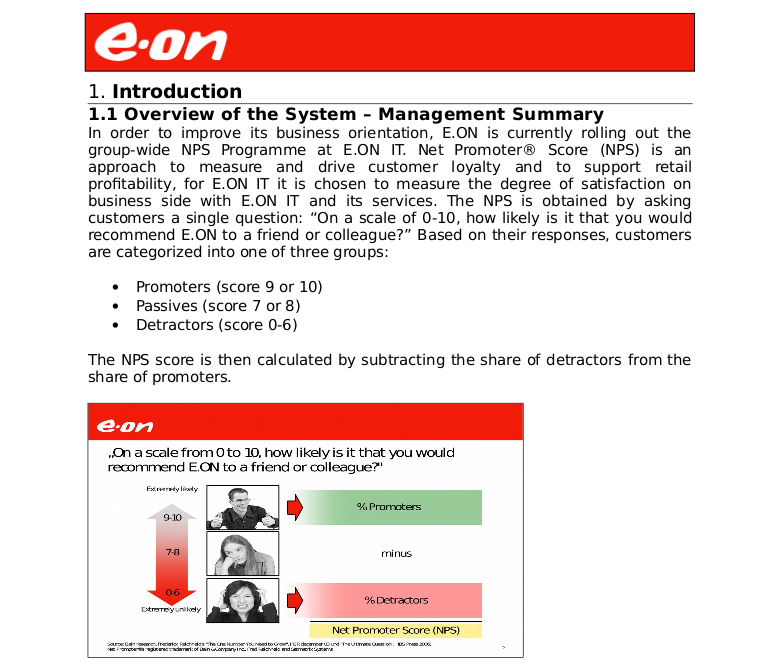
\includegraphics[scale=0.5]{BOR}
\caption{Primo caitolo del B.O.R. di NPS EBS}
\label{bor}
\end{center}
\end{figure}
\FloatBarrier

Questo documento mi ha permesso di avere una visione d'insieme su NPS, che ho descritto nel dettaglio nel \hyperref[cap:progetto-stage]{Capitolo 2}, e su quello che il cliente al tempo aveva richiesto. In questo modo ho potuto notare alcune differenze che ci sono rispetto all'ultima versione, e che poi ho ritrovato evidenziate nel secondo documento che ho visionato, ovvero il B.B.P.\footnotemark[3]
\footnotetext[3]{Per chiarimenti sulla documentazione vedere la \hyperref[fasi progetto]{Sezione 1.4.2}} 
del così detto \textit{sprint} 3, le cui pagine, strutturate come nella \hyperref[bbp]{Figura 3.4}, contengono per l'appunto le ultime \acrshort{cr} e le nuove funzionalità che sono state richieste dal committente e che sono state implementate prima del mio arrivo in azienda.

\begin{figure}[h!]
\begin{center}
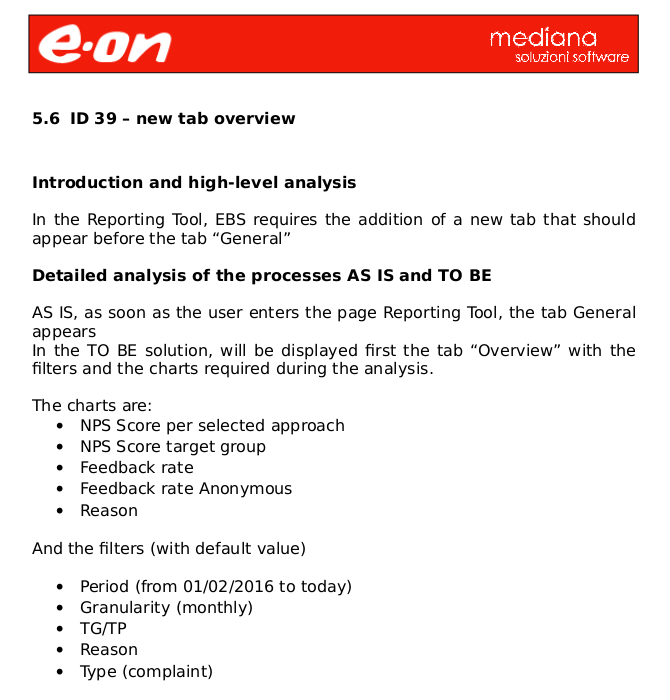
\includegraphics[scale=0.5]{BBP}
\caption{Esempio di soluzione proposta nel B.B.P. sprint 3 di NPS EBS}
\label{bbp}
\end{center}
\end{figure}
\FloatBarrier

Essendo arrivati ormai nel periodo conclusivo di questo \textit{sprint}, come dicevo precedentemente, non ho potuto assistere di persona a diversi passaggi di natura consulenziale, come tutta la fase di analisi e di pianificazione fino alla stesura stessa del B.B.P., ma per lo meno recuperando questa documentazione sono riuscito a capire meglio la situazione in cui il progetto si trovava. %\\

\subsection{Test e tracciamento dei bug}
\label{test}
A questo punto il mio tutor ha definito gli U.A.T. all'interno di un \textit{file} Excel condiviso su \textit{Google Drive} che io ho utilizzato sia per comprendere meglio tutte le modifiche che erano state proposte nel B.B.P. sia che per il loro scopo principale, ovvero verificare che le funzionalità dell'applicativo che sono state modificate, funzionassero effettivamente nel modo corretto. \\
Nelle figure \hyperref[indice UAT]{3.5} e \hyperref[test case]{3.6} si possono vedere alcuni esempi di come sono strutturate le pagine di questo \textit{test book}.

\begin{figure}[h!]
\begin{center}
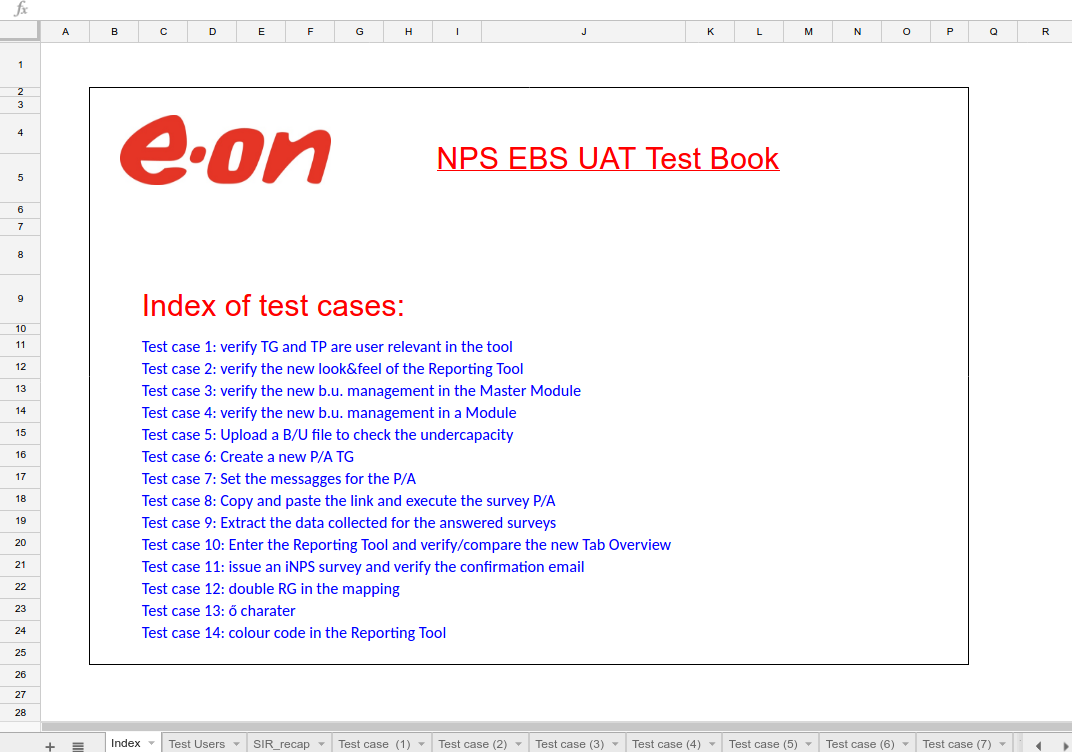
\includegraphics[scale=0.34]{indiceUAT}
\caption{Indice degli U.A.T per NPS EBS}
\label{indice UAT}
\end{center}
\end{figure}
\FloatBarrier

\begin{figure}[h!]
\begin{center}
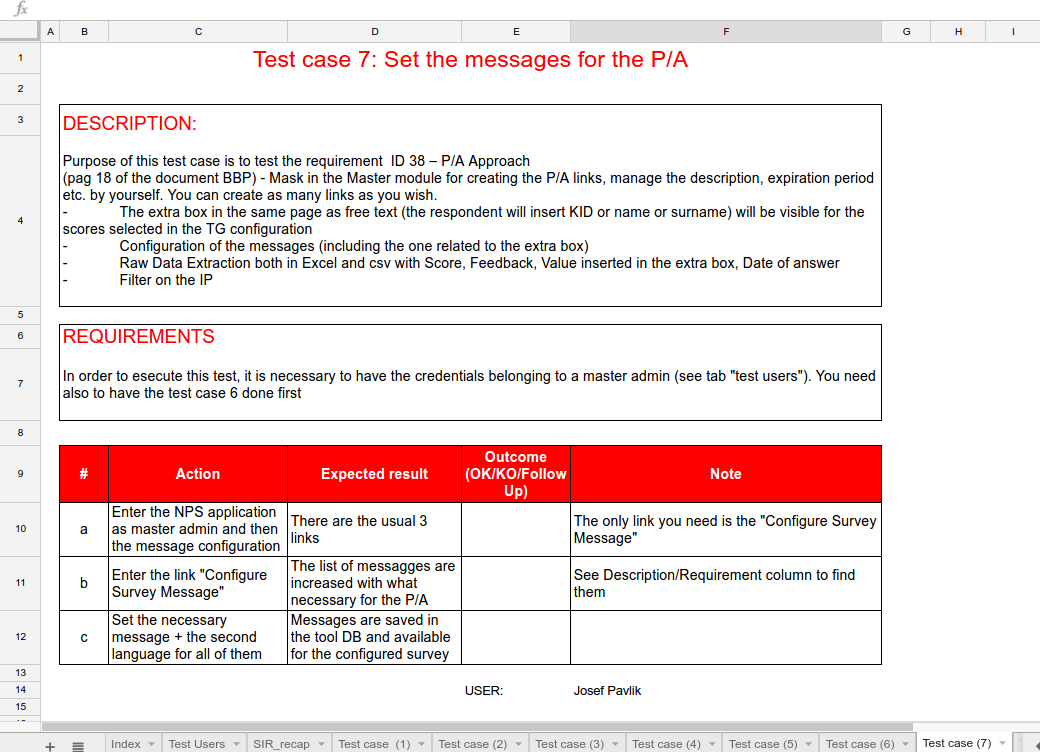
\includegraphics[scale=0.34]{testcaseUAT}
\caption{Esempio di U.A.T per NPS EBS}
\label{test case}
\end{center}
\end{figure}
\FloatBarrier

Successivamente anche il responsabile dell'azienda committente ha utilizzato il medesimo \textit{file} per testare il \textit{software} e per questo motivo a lui è stato riservato un particolare foglio chiamato SIR recap, nel quale ha potuto segnalare i \textit{bug} riscontrati assegnando ad essi diverse priorità (nella \hyperref[sir]{Figura 3.7} si può vedere una parte della lista da lui stilata).

\begin{figure}[h!]
\begin{center}
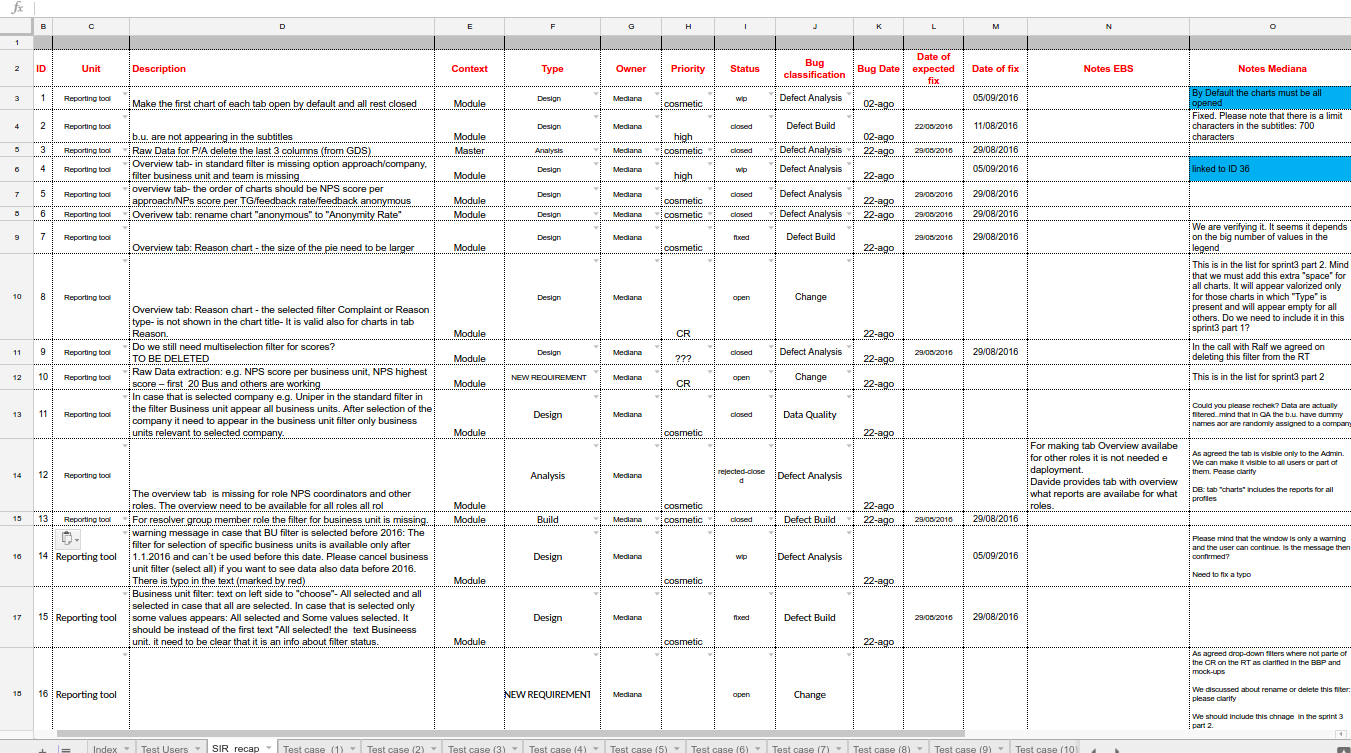
\includegraphics[scale=0.26]{SIR}
\caption{SIR recap compilato dal committente}
\label{sir}
\end{center}
\end{figure}
\FloatBarrier

Ognuna qualvolta veniva riscontrato un \textit{bug}, sia che esso venisse segnalato dal committente nel SIR recap sia che venisse individuato da me o il mio tutor, noi consulenti avevamo il compito di aggiungerlo come \textit{task} su un foglio di calcolo, riservato ai soli membri del \textit{team} che hanno seguito questo progetto. Questi \textit{bug} venivano assegnati agli sviluppatori che avevano il compito di cambiare lo stato dei \textit{task} segnalati come \textit{OPEN}, in \textit{WIP} (\emph{Work In Progess}) o \textit{CLOSED} a seconda del caso in cui essi ci avessero iniziato a lavorare o se lo avessero completato. Le altre colonne presenti in questa tabella identificano le date nelle quali venivano riscontrati i \textit{bug}, quelle di presunto rilascio e quelle di effettivo completamento. Ad ogni \textit{bug} veniva infine associata una descrizione, la pagina dell'applicativo corrispondente e una priorità a seconda di quanto fosse grave. \\ Utilizzandolo in questo modo, il \textit{file} Excel, del quale è possibile vedere una parte nella \hyperref[bug-report]{Figura 3.8}, andava ad assumere a tutti gli effetti lo stesso valore di un qualsiasi \gls{sistema di ticketing}.

\newpage
\begin{figure}[h!]
\begin{center}
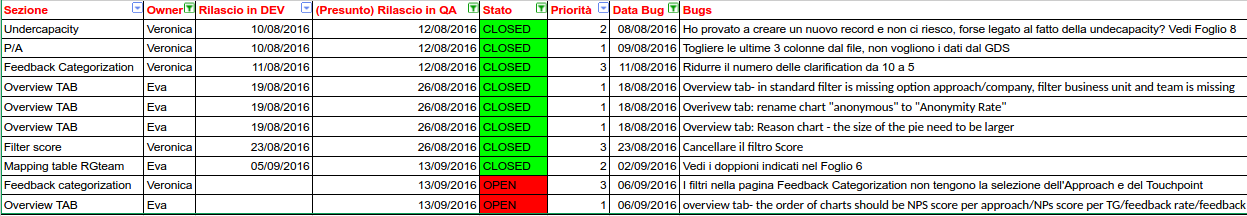
\includegraphics[scale=0.29]{Ticketing}
\caption{Foglio di calcolo utilizzato come sistema di ticketing}
\label{bug-report}
\end{center}
\end{figure}
\FloatBarrier

Fino ad avvenuto rilascio in PROD dell'applicativo, non è bastata un unica verifica delle funzionalità ma anzi, ad ogni nuovo rilascio in QA delle correzioni effettuate, ho ripetuto tutti gli U.A.T. dall'inizio in modo da verificare che a tutti gli effetti le modifiche fossero consistenti e che quindi i \textit{bug} fossero stati definitivamente risolti. Ciò è servito inoltre a verificare che non si fossero generate nuove situazione erronee dovute ai cambiamenti effettuati al codice o al passaggio di ambiente, nel quale qualcosa poteva non essere andata nel verso giusto.

\subsection{Manualistica}
\label{manuali}
Nell'ultima parte di questa prima fase di stage sono infine stato incaricato di un compito molto importante, ovvero correggere e ampliare, con le modifiche effettuate e le nuove funzionalità, tutti i manuali per ognuno dei ruoli esistenti all'interno di NPS. Questi ultimi differiscono fra loro in base agli incarichi che gli utenti hanno all'interno del sistema, dovuti al fatto che esistono diverse responsabilità o aree di pertinenza (geografiche o professionale) in EBS. \\
Durante la ristesura dei manuali, oltre a descrivere testualmente i vari passaggi che andavano svolti, ho aggiunto per ogni nuova funzione degli \gls{screenshot}, che consentono all'utente di individuare più chiaramente dove vanno applicate queste particolari azioni, come è stato fatto per esempio nella sezione che viene riportata nella \hyperref[manuale]{Figura 3.9}.

\begin{figure}[h!]
\begin{center}
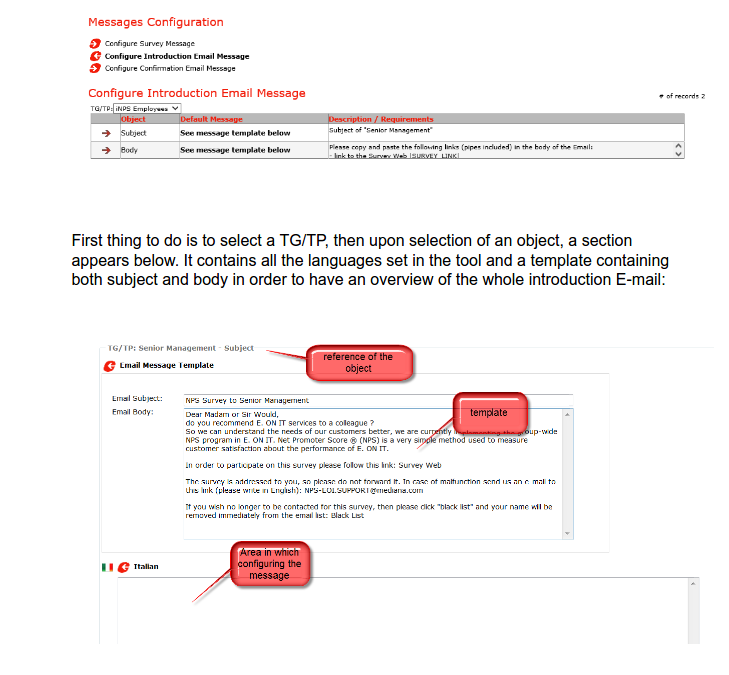
\includegraphics[scale=0.5]{manuale}
\caption{Pagina di un manuale contenente uno screenshot chiarificante}
\label{manuale}
\end{center}
\end{figure}
\FloatBarrier
 
\newpage
\section{Seconda fase di stage}
\label{seconda fase}
Per quanto riguarda la seconda parte dello stage, essa è collegata strettamente al fatto che molto spesso sorgevano \textit{bug} e piccole incongruenze rispetto le attese del committente, che prontamente ci segnalava sia tramite il già citato SIR recap che tramite \textit{e-mail}. \\
Per questo motivo, vista la grande mole di lavoro da gestire e dato che il \textit{team} di NPS si era visto privare di uno sviluppatore, a causa di impegni più prioritari in altri progetti, sono stato affiancato all'unica collega che al momento si stava occupando di fare \textit{support} al cliente EBS. Aggiungendo a questi momenti di pratica alcuni fasi di studio delle tecnologie C\#\footnotemark[4] e ASP.NET\footnotemark[4]
\footnotetext[4]{Tecnologie di cui ho già parlato nella \hyperref[tecnologie]{Sezione 1.5.2}}, sono riuscito a comprendere meglio il codice di NPS potendo così essere d'aiuto nelle settimane successive. 

\subsection{Estrazione di file Excel}
Tra i \textit{task} che mi sono stati assegnati durante la fase di \textit{support}, il più rilevante e allo stesso tempo quello che mi ha occupato più tempo è stato sicuramente l'estrazione dei dati in Excel. \\
In pratica, il problema derivava dal fatto che negli \textit{sprint} precedenti, NPS utilizzava per le estrazione di qualsiasi tipo di dati (come per esempio i feedback categorizzati, i dati degli utenti iscritti al sistema, le anagrafiche dei destinatari delle \textit{survey}, ecc.) una metodologia ormai deprecata. Infatti con gli aggiornamenti del pacchetto \textit{Microsoft Office} dalla versione 2010 in poi, il formato .xls che veniva costruito all'interno del programma, una volta estratto non veniva più riconosciuto dalle macchine del cliente, che era quindi impossibilitato a visualizzare le tabella alle quali era interessato. \\ Quindi, dopo aver analizzato per bene la situazione ed aver effettuato alcune ricerche, ho scoperto l'esistenza di \textbf{ClosedXML} (logo nella \hyperref[closedXML]{Figura 3.10}), una libreria scritta in C\# compatibile con tutti i linguaggi .NET che permette di generare \textit{file} nel più recente formato .xlsx. 

\begin{figure}[ht]
\begin{center}

\includegraphics[height=45pt]{ClosedXML}
\caption{Logo ClosedXML}
\label{closedXML}
\end{center}
\end{figure}

Come è possibile intuire dai nomi evidentemente antitetici, questa libreria nasce con l'obbiettivo di semplificare quanto è possibile fare con l'\acrshort{sdk}, proprietaria di \textit{Microsoft}, OpenXML, automatizzando operazioni inutilmente pesanti come la manipolazioni dei \textit{file} XML, di cui i documenti Excel sono composti. \\
Ho deciso di utilizzare questa libreria a discapito di altre anche perché è \textit{open surce} (licenza MIT), completamente gratuita e ben documentata; inoltre è possibile personalizzare a piacimento alcuni aspetti delle tabelle, tra i quali l'aggiunta di intestazioni e filtri alle colonne, la cui larghezza può essere impostata in modo che essa si adatti a seconda del suo contenuto. \\
Tutte queste caratteristiche mi hanno permesso di strutturare le varie tabelle come quella rappresentata nella \hyperref[tabella]{Figura 3.11} \\
Dopo aver importato il \textit{file} ClosedXML.dll all'interno del progetto ASP.NET di NPS, mi è infatti bastato aggiungere in ogni funzione di estrazione, definite all'interno delle classi che costituiscono l'applicativo, le seguenti righe di codice:

\newpage
\lstset{style=sharpc}
\begin{lstlisting}
var wb = new XLWorkbook();

// Aggiungo la DataTable creata precedentemente come un worksheet
wb.Worksheets.Add(dataTable);

wb.SaveAs("AddingDataTableAsWorksheet.xlsx");
\end{lstlisting}


Infatti l'ultima ma non meno importate delle motivazioni che mi hanno spinto a scegliere questa libreria è stata la perfetta compatibilità con gli oggetti di tipo \emph{Datatable}, che venivano già utilizzati in precedenza dentro a NPS e che vengono tuttora popolati dalle \gls{stored procedure} definite all'interno di SQL Server\footnotemark[5]
\footnotetext[5]{Ambiente di sviluppo già discusso nella \hyperref[ambienti sviluppo]{Sezione 1.5.3}}. 

\begin{figure}[h!]
\begin{center}
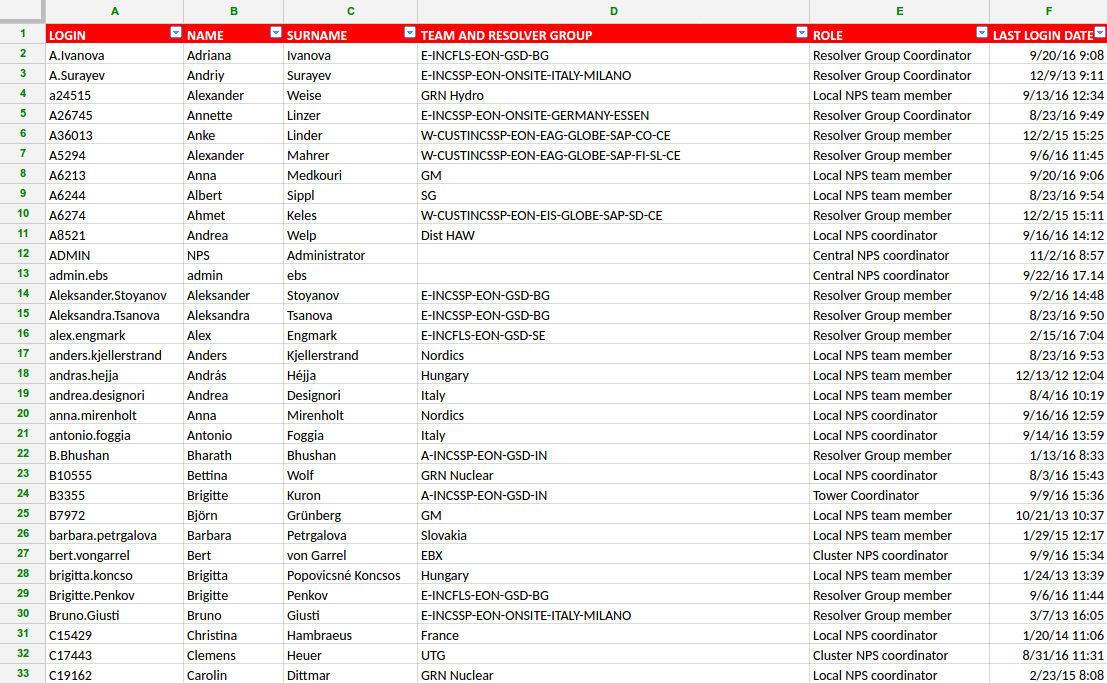
\includegraphics[scale=0.33]{UserList}
\caption{Esempio di Excel estratto contenente gli account registrati in NPS}
\label{tabella}
\end{center}
\end{figure}
\FloatBarrier


\subsection{L'importanza del database}
\label{db}
Come per tutte le applicazioni principali di Mediana S.r.l.u., anche NPS, o meglio CSIndex\footnotemark[6],
\footnotetext[6]{Nome del software così come viene venduto, come già detto nella \hyperref[prodotti]{Sezione 1.3}} è stato pensato per essere riadattabile alle esigenze di ogni nuovo cliente che lo desidera per la propria azienda. Per permettere ciò il \textit{database} è stato strutturato in modo che venga permessa la personalizzazione di ogni singolo aspetto delle varie pagine che compongono il programma, mentre la logica resta praticamente invariata, salvo quando ci sono delle nuove funzionalità non previste nella versione di base. Ciò è stato pensato anche per permettere agli sviluppatori di effettuare il più rapidamente possibile alcune modifiche che vengono richieste dal committente senza che ci sia il bisogno di effettuare ogni volta un \gls{deployment} del programma. \newpage
E in effetti così è stato anche nel mio caso, come per esempio quando mi è stato chiesto di ristrutturare il Reporting Tool\footnotemark[7]
\footnotetext[7]{Pagina dell'applicativo descritta nella \hyperref[reporting tool]{Sezione 2.3.3}}per determinati ruoli, aggiungendo o rimuovendo grafici, filtri e le diverse schede di cui esso è composto. Per fare ciò infatti, mi è bastato semplicemente aggiungere dei \textit{record} alle tabelle che permettessero di creare delle corrispondenze tra i ruoli e gli oggetti grafici descritti prima o, nel caso questi legami esistessero già, attivare dei \textit{flag} (corrispondenti ai valori 0 o 1 in una apposita colonna) per abilitarne la visualizzazione.   \\
Altro punto cardine per questo tipo di programmazione è l'implementazione di \gls{stored procedure} per manipolare ed estrarre i dati direttamente all'interno di SQL Server. Alcune di queste però non erano esenti da imperfezioni che hanno causato diversi \textit{bug}, come per esempio alcuni errori che si generavano durante la fase di estrazione oppure l'esistenza di incongruenze fra i dati estratti e quelli visualizzati all'interno dell'applicativo. In ogni caso comunque errori dovuti quasi sempre a sviste o casi limite non gestiti, risolvibili quindi con dei semplici accorgimenti.             % Kick-Off
%% !TEX encoding = UTF-8
% !TEX TS-program = pdflatex
% !TEX root = ../tesi.tex
% !TEX spellcheck = it-IT

%**************************************************************
\chapter{Analisi dei requisiti}
\label{cap:analisi-requisiti}
%**************************************************************

\intro{Breve introduzione al capitolo}\\

\section{Casi d'uso}

Per lo studio dei casi di utilizzo del prodotto sono stati creati dei diagrammi.
I diagrammi dei casi d'uso (in inglese \emph{Use Case Diagram}) sono diagrammi di tipo uml dedicati alla descrizione delle funzioni o servizi offerti da un sistema, così come sono percepiti e utilizzati dagli attori che interagiscono col sistema stesso.
Essendo il progetto finalizzato alla creazione di un tool per l'automazione di un processo, le interazioni da parte dell'utilizzatore devono essere ovviamente ridotte allo stretto necessario. Per questo motivo i diagrammi d'uso risultano semplici e in numero ridotto.

\begin{figure}[!h] 
    \centering 
    \includegraphics[width=0.9\columnwidth]{usecase/scenario-principale} 
    \caption{Use Case - UC0: Scenario principale}
\end{figure}

\begin{usecase}{0}{Scenario principale}
\usecaseactors{Sviluppatore applicativi}
\usecasepre{Lo sviluppatore è entrato nel plug-in di simulazione all'interno dell'IDE}
\usecasedesc{La finestra di simulazione mette a disposizione i comandi per configurare, registrare o eseguire un test}
\usecasepost{Il sistema è pronto per permettere una nuova interazione}
\label{uc:scenario-principale}
\end{usecase}

\section{Tracciamento dei requisiti}

Da un'attenta analisi dei requisiti e degli use case effettuata sul progetto è stata stilata la tabella che traccia i requisiti in rapporto agli use case.\\
Sono stati individuati diversi tipi di requisiti e si è quindi fatto utilizzo di un codice identificativo per distinguerli.\\
Il codice dei requisiti è così strutturato R(F/Q/V)(N/D/O) dove:
\begin{enumerate}
	\item[R =] requisito
    \item[F =] funzionale
    \item[Q =] qualitativo
    \item[V =] di vincolo
    \item[N =] obbligatorio (necessario)
    \item[D =] desiderabile
    \item[Z =] opzionale
\end{enumerate}
Nelle tabelle \ref{tab:requisiti-funzionali}, \ref{tab:requisiti-qualitativi} e \ref{tab:requisiti-vincolo} sono riassunti i requisiti e il loro tracciamento con gli use case delineati in fase di analisi.

\newpage

\begin{table}%
\caption{Tabella del tracciamento dei requisti funzionali}
\label{tab:requisiti-funzionali}
\begin{tabularx}{\textwidth}{lXl}
\hline\hline
\textbf{Requisito} & \textbf{Descrizione} & \textbf{Use Case}\\
\hline
RFN-1     & L'interfaccia permette di configurare il tipo di sonde del test & UC1 \\
\hline
\end{tabularx}
\end{table}%

\begin{table}%
\caption{Tabella del tracciamento dei requisiti qualitativi}
\label{tab:requisiti-qualitativi}
\begin{tabularx}{\textwidth}{lXl}
\hline\hline
\textbf{Requisito} & \textbf{Descrizione} & \textbf{Use Case}\\
\hline
RQD-1    & Le prestazioni del simulatore hardware deve garantire la giusta esecuzione dei test e non la generazione di falsi negativi & - \\
\hline
\end{tabularx}
\end{table}%

\begin{table}%
\caption{Tabella del tracciamento dei requisiti di vincolo}
\label{tab:requisiti-vincolo}
\begin{tabularx}{\textwidth}{lXl}
\hline\hline
\textbf{Requisito} & \textbf{Descrizione} & \textbf{Use Case}\\
\hline
RVO-1    & La libreria per l'esecuzione dei test automatici deve essere riutilizzabile & - \\
\hline
\end{tabularx}
\end{table}%             % Concept Preview
%% !TEX encoding = UTF-8
% !TEX TS-program = pdflatex
% !TEX root = ../tesi.tex
% !TEX spellcheck = it-IT

%**************************************************************
\chapter{Progettazione e codifica}
\label{cap:progettazione-codifica}
%**************************************************************

\intro{Breve introduzione al capitolo}\\

%**************************************************************
\section{Tecnologie e strumenti}
\label{sec:tecnologie-strumenti}

Di seguito viene data una panoramica delle tecnologie e strumenti utilizzati.

\subsection*{Tecnologia 1}
Descrizione Tecnologia 1.

\subsection*{Tecnologia 2}
Descrizione Tecnologia 2

%**************************************************************
\section{Ciclo di vita del software}
\label{sec:ciclo-vita-software}

%**************************************************************
\section{Progettazione}
\label{sec:progettazione}

\subsubsection{Namespace 1} %**************************
Descrizione namespace 1.

\begin{namespacedesc}
    \classdesc{Classe 1}{Descrizione classe 1}
    \classdesc{Classe 2}{Descrizione classe 2}
\end{namespacedesc}


%**************************************************************
\section{Design Pattern utilizzati}

%**************************************************************
\section{Codifica}
             % Product Prototype
%% !TEX encoding = UTF-8
% !TEX TS-program = pdflatex
% !TEX root = ../tesi.tex
% !TEX spellcheck = it-IT

%**************************************************************
\chapter{Verifica e validazione}
\label{cap:verifica-validazione}
%**************************************************************             % Product Design Freeze e SOP
% !TEX encoding = UTF-8
% !TEX TS-program = pdflatex
% !TEX root = ../tesi.tex
% !TEX spellcheck = it-IT

%**************************************************************
\chapter{Conclusioni}
\label{cap:conclusioni}
%**************************************************************
\section{Consuntivo finale}
\label{consuntivo}
A differenza di quanto riportato dal calendario delle attività svolte durate lo stage, descritte nella \hyperref[calendario]{Sezione 3.2}, il piano di lavoro proposto inizialmente era molto generico definendo solamente delle fasi di massima in modo da lasciare spazio ad eventuali future modifiche o aggiunte:

\begin{enumerate}
\item \textbf{Settimana 1}: introduzione in azienda e condivisione \textit{password} aziendali;
\item \textbf{Settimana 2}: introduzione ai prodotti aziendali e condivisione manuali e documentazione riferiti ai prodotti di punta dell'azienda;
\item \textbf{Settimana 3}: formazione sui prodotti XE\footnotemark[1] e XC\footnotemark[1] legati alla fatturazione dell'energia elettrica;
\footnotetext[1]{Abbreviazioni dei prodotti XEnergy e XContract discussi nella \hyperref[prodotti]{Sezione 1.3}} 
\item \textbf{Settimana 4-5}: focalizzazione sul prodotto CSIndex ed esecuzione di test funzionali sulla nuova versione del \textit{software} (NPS EBS) in affiancamento al tutor;
\item \textbf{Settimana 6-7}: manualistica, U.A.T\footnotemark[2],
\footnotetext[2]{Test visti nella \hyperref[fasi progetto]{Sezione 1.4.2}} \textit{roll out} del progetto NPS EBS;
\item \textbf{Settimana 8}: verifica dell'apprendimento degli obiettivi prefissati.
\end{enumerate}

Per avere una visione d'insieme delle attività inizialmente pianificate, riporto il corrispondente \gls{diagramma di Gantt} nella \hyperref[gantt pianificazione]{Figura 4.1}.

\begin{figure}[h!]
\begin{center}
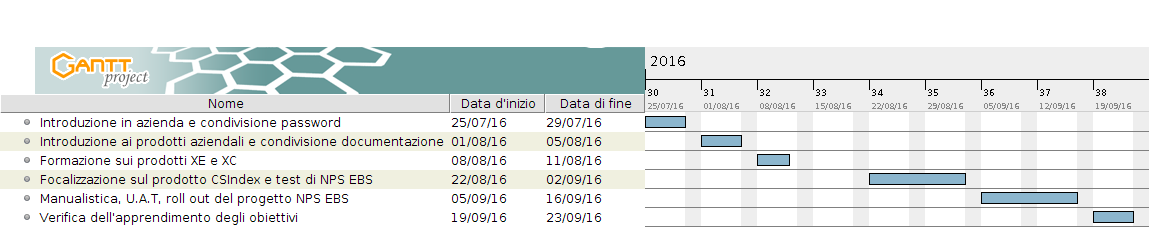
\includegraphics[scale=0.32]{GanttPianificazione} 
\caption{Diagramma di Gantt delle attività che erano state pianificate}
\label{gantt pianificazione}
\end{center}
\end{figure}
\FloatBarrier

\newpage
Le cause principali che hanno spinto a cambiare il piano di lavoro proposto, sono ricollegabili soprattutto al fatto che sono sorti dei rischi che non erano stati calcolati o per meglio dire delle situazioni imprevedibili come le dimissioni di una collega che risultava essere una delle figure di riferimento per alcuni clienti considerati molto importanti nel contesto aziendale. \\
Questo fatto ha attirato l'attenzione di tutto il personale proprio al momento del mio arrivo in Mediana S.r.l.u., con malumori dovuti a continue riunioni per effettuare imminenti e problematici passaggi di consegne del lavoro che la collega stava svolgendo per i progetti che in parte avrebbero dovuto coinvolgermi (XE e XC). \\
Per questo motivo il mio tutor ha giustamente preferito focalizzare il mio stage soltanto su NPS EBS, preferendo rimandare ad un possibile futuro la mia formazione sugli altri prodotti, sui quali mi è stata fatta solamente una breve panoramica. \\
Quindi essendo di fatto saltata la pianificazione della seconda e terza settimana ed essendo state largamente sovrastimate alcune fra le attività restanti, piuttosto che continuare a svolgere gli stessi incarichi, che iniziavano ad essere troppo ripetitivi e per questo non più molto istruttivi, ho deciso, in accordo con il tutor interno e il tutor aziendale, di cogliere l'opportunità di prendere un posto lasciato vacante da sviluppatore, come avevo già anticipato nella \hyperref[seconda fase]{Sezione 3.5}, non appena questo si è liberato. 

\section{Raggiungimento degli obiettivi}
Gli obiettivi che erano stati delineati sono da considerarsi quasi tutti superati, nonostante il cambiamento che c'è stato nella pianificazione. Infatti, trattandosi più che altro di un progetto formativo, gli obiettivi non erano del tutto concreti, ma fungevano più che altro da linea guida da seguire per riuscire ad essere introdotto al meglio nella realtà aziendale di Mediana S.r.l.u e nel lavoro da consulente dando allo stesso tempo uno sguardo ad un possibile futuro in questo ambito, tramite un inserimento nell'organico per un periodo più lungo delle canoniche 8 settimane di stage nel caso entrambi le parti fossero uscite da questa esperienza in maniera positiva.
Nella \hyperref[tabella obiettivi]{Tabella 4.1} riporto la lista degli obiettivi già visti nella \hyperref[obiettivi]{Sezione 1.1}, specificando per ognuno di essi le ragioni per le quali possano essere considerati come raggiunti o meno.

\newpage
\normalsize
\begin{longtable}{|>{\centering}m{6cm}|m{6cm}<{\centering}|}
\hline
\textbf{Obiettivo} & \textbf{Raggiungimento}\\
\hline
\endhead
{Conoscenza degli applicativi di Mediana S.r.l.u., in particolare di CSIndex nella sua ultima versione NPS EBS} & {\textbf{Parzialmente raggiunto}: a discapito di una più approfondita conoscenza del \textit{software} NPS EBS, che come spiegato più volte si rifà al più generico CSIndex, e a causa di un evento non prevedibile, come discusso nella \hyperref[consuntivo]{Sezione 4.1}, purtroppo è stata accantonata l'idea di farmi conoscere gli altri prodotti offerti da Mediana S.r.l.u.} 
\\ \hline

{Conoscenza delle fasi consulenziali come:
	\begin{itemize}
	\item Redazione di \textit{test book} per U.A.T.\footnotemark[1];
	\item Test e verifiche dei programmi presi in esame;
	\item Redazione di manuali propedeutici al \textit{roll out} dell'applicativo.
	\end{itemize}} & {\textbf{Interamente raggiunto}:  incarichi appresi tutti durante la prima metà dello stage, descritta nella \hyperref[prima fase]{Sezione 3.4}}
\\ \hline

{Apprendimento del \gls{data model} di NPS EBS} & {\textbf{Interamente raggiunto}: ho imparato a conoscere il \gls{data model} di NPS sia teoricamente durante la fase di test e stesura dei manuali, rispettivamente \hyperref[test]{Sezione 3.4.2} e \hyperref[manuali]{Sezione 3.4.3}, che più approfonditamente nella seconda metà dello stage, descritta nella \hyperref[seconda fase]{Sezione 3.5}, quando ho potuto mettere le mani al codice}
\\ \hline

{Sviluppare una buona autonomia nella progettazione e sviluppo di \textit{statement} SQL} & {\textbf{Interamente raggiunto}: in parte già presente nel mio bagaglio culturale poiché si tratta di una capacità che ho appreso durante il corso di Basi di Dati, è stata sicuramente rafforzata in base alle esigenze avute durante la seconda metà dello stage quando ho dovuto esplorare il database di NPS per risolvere alcuni bug, come ho descritto nella \hyperref[db]{Sezione 3.4.2}}
\\ \hline

\caption[Tabella Requisiti Implementati]{Tabella Requisiti Implementati}
\label{tabella obiettivi}
\end{longtable}

%**************************************************************
\newpage
\section{Conoscenze acquisite}
L'esperienza di stage effettuata ha contribuito sicuramente ad ampliare le mie conoscenze professionali. \\
In particolare avendo avuto l'occasione di provare, anche se solo in parte, gli impieghi di un consulente tecnico, sono riuscito a comprendere le dinamiche di un lavoro che prima di allora non avevo mai preso in considerazione. \\
Allo stesso tempo però il fatto di essere riuscito a occupare una parte di stage come sviluppatore, anche se soltanto effettuando semplici operazioni di \textit{bug-fixing}, mi ha permesso di arricchire le mie conoscenze informatiche con lo studio di tecnologie mai utilizzate in precedenza, come C\# e ASP.NET, delle quali ho già avuto modo di parlare nella \hyperref[tecnologie]{Sezione 1.5.2}. \\
Oltre alle conoscenze tecniche appena descritte, l'attività di stage mi ha
permesso soprattutto di entrare in ottica aziendale potendo così imparare a relazionarmi al meglio con i colleghi e a collaborare con loro per uno stesso obiettivo. \\
Prima di allora infatti non avevo mai avuto modo di misurare le mie capacità in ambito
lavorativo e grazie a quest'esperienza ho potuto notare, rispetto ai progetti svolti durante i corsi universitari, alcune nette differenze nella gestione di un progetto. Mi riferisco soprattutto al fatto che si tende a voler rilasciare un prodotto nel minor tempo possibile piuttosto che puntare ad avere una buona qualità ed affidabilità che si va invece ad ottenere man mano nel tempo attraverso lunghe fasi di \textit{support}. Ciò è dovuto probabilmente al fatto che esistono profonde differenze tra gli obiettivi che ci sono nel mondo del lavoro e quelli presenti nell'ambiente accademico. Infatti, per le aziende, ciò che alla fine conta veramente è ottenere un profitto nel minor tempo possibile. 

%**************************************************************
\section{Valutazione personale}
Nel complesso posso dire che l'esperienza di stage è stata molto interessante e costruttiva e anche se il fatto di poter lavorare come consulente ad un progetto diverso dai classici canoni mi allettava, col senno di poi posso affermare che questo genere di impiego si è rivelato non essere il più adatto per me anche perché non ha potuto valorizzare le conoscenze e competenze acquisite durante il percorso di studio effettuato presso la facoltà di Informatica. Infatti non appena ho iniziato a lavorare come sviluppatore mi sono sentito sin da subito molto più a mio agio, tanto è vero che ho deciso di accettare la proposta di prolungare questa esperienza in Mediana S.r.l.u. affrontandola questa volta nel modo a me più congeniale, mettendo comunque a disposizione le conoscenze consulenziali che ho appreso durante lo stage nel caso ci fosse il bisogno di farlo.\\
L'esperienza di stage è stata inoltre molto positiva sul piano umano e relazionale, infatti nonostante il difficile periodo iniziale nel quale l'azienda si è ritrovata, il gruppo di Mediana S.r.l.u. si è rivelato essere come una grande famiglia dove ci si aiuta l'un l'altro ogni volta che qualcuno è in difficoltà o ha un dubbio da chiarire, potendo vivere così le giornate lavorative in un clima tranquillo e sereno. In linea con quello appena detto, devo ringraziare in particolar modo il mio tutor, che ha avuto il difficile compito di guidarmi passo dopo passo attraverso questo percorso, per me del tutto nuovo. \\
Alla luce di tutto ciò mi sento di dire che l'esperienza in sé è stata molto utile poiché mi ha permesso di entrare in contatto diretto con quello che rappresenta la realtà lavorativa e tutte le problematiche che ne derivano; cosa molto importante visto che a mio parere non è possibile apprenderla all'interno del mondo universitario. \newpage
In conclusione posso comunque affermare che il corso di laurea triennale in Informatica dell'Università di Padova offre un'ottima preparazione che permette di affrontare le più diverse situazioni, analizzandole in modo critico, però soltanto sfruttando questa opportunità di stage che ci viene offerta si ha la concreta possibilità di colmare le lacune rimaste venendo di fatto introdotti all'interno del mondo lavorativo.
             % Conclusioni
\appendix                               
% !TEX encoding = UTF-8
% !TEX TS-program = pdflatex
% !TEX root = ../tesi.tex
% !TEX spellcheck = it-IT

%**************************************************************
\chapter{Convenzioni tipografiche}
%**************************************************************

Riguardo la stesura del testo, relativamente al documento sono state adottate le seguenti convenzioni tipografiche:
\begin{itemize}
	\item Gli acronimi, le abbreviazioni e i termini ambigui o di uso non comune menzionati sono evidenziati dal colore blu e quindi definiti nel glossario, situato alla fine del presente documento;
	\item Tutti i riferimenti a capitoli, sezioni o figure presenti all'interno dell'elaborato sono anch'essi evidenziati in blu;
	\item I termini in lingua straniera o facenti parti del gergo tecnico sono marcati con il carattere corsivo;
	\item Le parole chiave di una determinata sezione sono scritte in grassetto;
	\item Negli elenchi puntati, per ogni punto, la prima parola presenta la prima lettera maiuscola;
    \item Negli elenchi puntati, in tutti i punti viene usato il punto e virgola per concludere, ad eccezione dell'ultimo che termina con un punto;
    \item Negli elenchi puntati quando si presenta un termine seguito dai due punti questo viene riportato in grassetto.
\end{itemize}

             % Appendice A

%**************************************************************
% Materiale finale
%**************************************************************
\backmatter
\printglossary[title={Glossario}]
\printglossary[type=\acronymtype,title={Acronimi}]
% !TEX encoding = UTF-8
% !TEX TS-program = pdflatex
% !TEX root = ../tesi.tex
% !TEX spellcheck = it-IT

%**************************************************************
% Bibliografia
%**************************************************************

\cleardoublepage
\chapter{Bibliografia}

\nocite{*}
%\printbibliography

\bibbycategory % equivale a dare un \printbibliography per ogni categoria


\end{document}